% -*- TeX-master: "main" -*-

\section{Package syntax and semantics}
\label{sec:syntax}
This section contains a definition of the syntax and semantics of the Spatial package for \sbmlthreecore.  The Spatial package involves several new object classes, and extends the existing \Model, \Compartment, \Species, \Reaction, and \Parameter object class.  \sec{examples} contains complete examples of using the constructs in SBML models.

%{\color{red} Lucian: \notice Periodically when I have comments, I'll put them in sections that look like this--in red, with the pointy-hand icon off to the side.  They tend to be design questions I had when creating this document for parts I thought were not clear, or are suggestions for changes that could be made.}


\subsection{Overview of spatial extension}
The SBML \Compartment, \Reaction and \Species, and molecular transport mechanisms (\DiffusionCoefficient, \AdvectionCoefficient, \BoundaryCondition) are mapped to geometric domains to describe spatial models within SBML.  The primary mechanism to accomplish this mapping is to simply map \Compartments to collections of geometric Domains called \DomainTypes.  Each \Domain is a contiguous patch of volumetric space or a contiguous surface patch that is ultimately described by a single system of equations (whichever mathematical framework is used).  In analogy with initial conditions, the mathematical system defined within a domain often needs a definition of what happens at the domain boundary (e.g. boundary conditions) to complete the specification.  Because of this, the boundaries between adjacent domains need to be identified so that appropriate boundary conditions can be specified.  For compactness of representation, rather than map to each individual \Domain, \Compartments are mapped to \DomainTypes, along with the corresponding \Species and \Reactions (with the new compartment attribute).

\subsubsection{Geometry}
The \Geometry object within a model is completely modular and does not reference the rest of the model, promoting reuse of the same geometry in different models.  The geometry separately defines a coordinate system, a list of domain types, a list of domains and their adjacency relationships, and a list of alternate geometric representations.

\subsubsection{Alternative \GeometryDefinitions}
Modeling and simulation tools will each natively support some subset (often just one) of the possible \GeometryDefinitions (analytic, sampled field, constructive solid geometry, parametric, or mixed shapes).  Interoperability will be enhanced if tools write as many geometry definitions as they are able.  Upon reading the model, a tool will typically choose the most convenient geometry definition, i.e. the one that it natively supports.  If a tool does not edit the geometry, it has the ability to preserve the alternate representations during model editing (because the mapping of the model to the geometry is not stored in the geometry).

There are two general classes of geometric representation specification: those that explicitly specify surfaces and those that implicitly specify surfaces.  For example, a level set is a field where a specific isosurface of the field specifies a geometric surface.  A geometry described using constructive solid geometry of geometric primitives (e.g. spheres, cylinders) specifies directly which points are "inside" an object.  Alternatively, explicit surface representations explicitly declare the set of points belonging to surfaces (e.g. polygonal tessellations).



% --------------------------------------------------------------------------
\subsection{Namespace URI and other declarations necessary for using this package}
\label{xml-namespace}
Every SBML Level~3 package is identified uniquely by an XML namespace URI.  For an SBML document to be able to use a given Level~3 package, it must declare the use of that package by referencing its URI.  The following is the namespace URI for this version of the Spatial package for \sbmlthreecore:
\begin{center}
\uri{http://www.sbml.org/sbml/level3/version1/spatial/version1}
\end{center}

In addition, SBML documents using a given package must indicate whether the package can be used to change the mathematical interpretation of a model.  This is done using the attribute \token{required} on the \token{<sbml>} element in the SBML document.  For the Spatial package, the value of this attribute must be \val{true}, because the use of the Spatial package can change the mathematical meaning of a model.

The following fragment illustrates the beginning of a typical SBML model using \sbmlthreecore and this version of the Spatial package:

\begin{example}
<?xml version="1.0" encoding="UTF-8"?>
<sbml xmlns="http://www.sbml.org/sbml/level3/version1/core" level="3" version="1"
      xmlns:spatial="http://www.sbml.org/sbml/level3/version1/spatial/version1"
      spatial:required="true">
\end{example}


\subsection{Primitive data types}
\label{new-primitive-types}

The Spatial package uses a number of the primitive data types described in Section~3.1 of the \sbmlthreecore specification, and adds several additional primitive types described below.


\subsubsection{Type \fixttspace\primtypeNC{SpId}}
\label{primtype-SpId}

The type \primtype{SpId} is derived from \primtype{SId}
(\sbmlthreecore specification Section~3.1.7) and has identical syntax. The \primtype{SpId} type is used as the data type for the identifiers of various objects in the Spatial Processes package.  The purpose of having a separate type for such identifiers is to enable the space of possible spatial identifier values to be separated from the space of all other identifier values in SBML.  The equality of \primtype{SpId} values is determined by an exact character sequence match; i.e., comparisons of these identifiers must be performed in a case-sensitive manner.


\subsubsection{Type \fixttspace\primtypeNC{SpIdRef}}
\label{primtype-SpIdRef}

Type \primtype{SpIdRef} is used for all attributes that refer to identifiers of type \primtype{SpId}.  It is derived from \primtype{SpId}, but with the restriction that the value of an attribute having type \primtype{SpIdRef} must match the value of a \primtype{SpId} attribute in the relevant model;  in other words, the value of the attribute must be an existing spatial identifier in the referenced model.  As with \primtype{SpId}, the equality of \primtype{SpIdRef} values is determined by exact character sequence match; i.e., comparisons of these identifiers must be performed in a case-sensitive manner.


\subsubsection{Type \fixttspace\primtypeNC{BoundaryConditionKind}}
\label{primtype-BoundaryConditionKind}

The \primtype{BoundaryConditionKind} primitive data type is used in the definition of the \BoundaryCondition class.  It is derived from type \primtype{string} and its values are restricted to being one of the following possibilities: \val{Neumann}, \val{Dirichlet}, \val{Robin\_valueCoefficient}, \val{Robin\_inwardNormalGradientCoefficient}, and \val{Robin\_sum}.  Attributes of type \primtype{BoundaryConditionKind} cannot take on any other values.  The meaning of these values is discussed in the context of the \BoundaryCondition class's definition in \sec{boundarycondition-class}.


\subsubsection{Type \fixttspace\primtypeNC{CoordinateKind}}
\label{primtype-CoordinateKind}

The \primtype{CoordinateKind} primitive data type is used in the definition of the \CoordinateComponent class.  It is derived from type \primtype{string} and its values are restricted to being one of the following possibilities: \val{cartesianX}, \val{cartesianY}, and \val{cartesianZ}.
%, \val{spherical\-Radius}, \val{sphericalAzimuth}, \val{sphericalElevation}, \val{cylindrical\-Radius}, \val{cylindricalAzimuth}, \val{cylindricalHeight}, \val{polarRadius}, and \val{polarAzimuth}.
Attributes of type \primtype{CoordinateKind} cannot take on any other values.  The meaning of these values is discussed in the context of the \CoordinateComponent class's definition in \sec{coordinatecomponent-class}.

Other \primtype{CoordinateKind} types are held in reserve for future versions of this specification, and may include \val{spher\-i\-cal\-Radius}, \val{sphericalAzimuth}, \val{sphericalElevation}, \val{cylindrical\-Radius}, \val{cylindricalAzimuth}, \val{cy\-lin\-dricalHeight}, \val{polarRadius}, and \val{polarAzimuth}.



%\subsubsection{Type \fixttspace\primtypeNC{CoordinateKind}}
%\label{primtype-coordinatekind}
%
%The \primtype{CoordinateKind} primitive data type is used in the definition of the \CoordinateComponent class.  The type \primtype{CoordinateKind} is derived from type \primtype{string} and its values are restricted to being one of the following possibilities: \val{normal}, \val{symmetrical}, and \val{fixed}.  Attributes of type \primtype{CoordinateKind} cannot take on any other values.  The meaning of these values is discussed in the context of the \CoordinateComponent class's definition in \sec{coordinatecomponent-class}.

\subsubsection{Type \fixttspace\primtypeNC{DataKind}}
\label{primtype-DataKind}

The \primtype{DataKind} primitive data type is used in the definition of the \SampledField and \ParametricGeometry classes.  It is derived from type \primtype{string} and its values are \changed{suggested to be limited to the following three options: \val{uint}, \val{int}, or \val{double}.  For backwards compatibility, and for space reasons, the values \val{float}, \val{uint8}, \val{uint16}, and \val{uint32} are also allowed.}  Attributes of type \primtype{DataKind} cannot take on any other values.  The meaning of these values is discussed in the context of the classes' definitions in \sec{sampledfield-class} and \sec{parametricgeometry-class}.


\subsubsection{Type \fixttspace\primtypeNC{DiffusionKind}}
\label{primtype-DiffusionKind}

The \primtype{DiffusionKind} primitive data type is used in the definition of the \DiffusionCoefficient class.  It is derived from type \primtype{string} and its values are restricted to being one of the following possibilities: \val{isotropic}, \val{anisotropic}, and \val{tensor}.  Attributes of type \primtype{DiffusionKind} cannot take on any other values.  The meaning of these values is discussed in the context of the \DiffusionCoefficient class's definition in \sec{diffusioncoefficient-class}.


\subsubsection{Type \fixttspace\primtypeNC{CompressionKind}}
\label{primtype-CompressionKind}

The \primtype{CompressionKind} primitive data type is used in the definition of the \SampledField and \ParametricObject classes.  It is derived from type \primtype{string} and its values are restricted to being one of the following possibilities: \val{uncompressed}, and \val{deflated}.  Attributes of type \primtype{CompressionKind} cannot take on any other values.  The meaning of these values is discussed in the context of the classes' definitions in \sec{spatialpoints-class}, \sec{parametricobject-class}, and \sec{sampledfield-class}.


\subsubsection{Type \fixttspace\primtypeNC{FunctionKind}}
\label{primtype-FunctionKind}

The \primtype{FunctionKind} primitive data type is used in the definition of the \AnalyticVolume class.  It is derived from type \primtype{string} and its values are restricted to being one of the single possibility \val{layered}.  Attributes of type \primtype{FunctionKind} cannot take on any other values.  The meaning of these values is discussed in the context of the \AnalyticVolume class's definition in \sec{analyticvolume-class}.


\subsubsection{Type \fixttspace\primtypeNC{GeometryKind}}
\label{primtype-GeometryKind}

The \primtype{GeometryKind} primitive data type is used in the definition of the \Geometry class.  It is derived from type \primtype{string} and its values are restricted to being the single possibility \val{cartesian}.  Other \primtype{GeometryKind} types are held in reserve for future versions of this specification, and may include \val{cylindrical}, \val{spherical}, and \val{polar}.  Attributes of type \primtype{GeometryKind} cannot take on any other values.  The meaning of these values is discussed in the context of the \Geometry class's definition in \sec{geometry-class}.


\subsubsection{Type \fixttspace\primtypeNC{InterpolationKind}}
\label{primtype-InterpolationKind}

The \primtype{InterpolationKind} primitive data type is used in the definition of the \SampledField class.  It is derived from type \primtype{string} and its values are restricted to being one of the following possibilities: \val{nearestNeighbor} and \val{linear}.  Attributes of type \primtype{InterpolationKind} cannot take on any other values.  The meaning of these values is discussed in the context of the \SampledField class's definition in \sec{sampledfield-class}.


\subsubsection{Type \fixttspace\primtypeNC{PolygonKind}}
\label{primtype-PolygonKind}

The \primtype{PolygonKind} primitive data type is used in the definition of the \ParametricObject class.  It is derived from type \primtype{string} and its values are restricted to being one of the following possibilities: \val{triangle} and \val{quadrilateral}.  Attributes of type \primtype{PolygonKind} cannot take on any other values.  The meaning of these values is discussed in the context of the \ParametricObject class's definition in \sec{parametricobject-class}.


\subsubsection{Type \fixttspace\primtypeNC{PrimitiveKind}}
\label{primtype-PrimitiveKind}

The \primtype{PrimitiveKind} primitive data type is used in the definition of the \CSGPrimitive class.  It is derived from type \primtype{string} and its values are restricted to being one of the following possibilities: \val{sphere}, \val{cube}, \val{cylinder}, and \val{cone}, for three-dimensional \CSGObject elements, and \val{circle}, and \val{square}, for two-dimensional \CSGObject elements.  Attributes of type \primtype{PrimitiveKind} cannot take on any other values.  The meaning of these values is discussed in the context of the \CSGPrimitive class's definition in \sec{sampledfield-class}.


\subsubsection{Type \fixttspace\primtypeNC{SetOperation}}
\label{primtype-SetOperation}

The \primtype{SetOperation} primitive data type is used in the definition of the \CSGSetOperator class.  It is derived from type \primtype{string} and its values are restricted to being one of the following possibilities: \val{union}, \val{intersection}, and \val{difference}.  Attributes of type \primtype{SetOperation} cannot take on any other values.  The meaning of these values is discussed in the context of the \CSGSetOperator class's definition in \sec{csgsetoperator-class}.


\subsubsection{Type \fixttspace\primtypeNC{doubleArray}}
\label{primtype-doubleArray}

The \primtype{doubleArray} primitive data type is a space-delimited list of \primtype{double} values in a single string.  

\subsubsection{Type \fixttspace\primtypeNC{arrayData}}
\label{primtype-arrayData}

The \primtype{arrayData} primitive data type is used in the definition of the \SampledField and \ParametricObject classes.  It consists of a possibly-compressed whitespace-and-semicolon-delimited list of numerical values in a single string.  The meaning and possible content of these values is discussed in the context of the classes' definitions in \sec{sampledfield-class} and \sec{parametricgeometry-class}.

%\clearpage


\subsection{The extended \Model object}
\label{extended-model-class}
The \Model object is extended in the spatial package to contain a new \Geometry child, as seen in
\fig{model-uml}. The \Geometry element is contained in the Model element in the 'spatial' namespace. In order to specify a spatial geometry, some of the existing SBML elements need to be extended (\Compartment, \Species, \Parameter, and \Reaction). These extensions to the SBML elements are discussed in the sections that follow.
 
\begin{figure}[ht]
  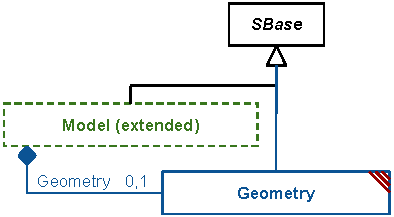
\includegraphics{figs/extended-model-uml}
  \caption{The definition of the extended \Model object from the Spatial package.  The \Geometry object and its children are defined in their own sections.}
  \label{model-uml}
\end{figure}




\subsection{The extended \Compartment object}
\label{extended-compartment-class}

The \Compartment in the SBML core is extended while defining a spatial model. An SBML model with spatial geometry defines domain types (classes of domains that are anatomically and physiologically similar). These domain types need to be mapped to a compartment in the SBML model. \Compartments are extended to define \CompartmentMappings that map compartments to \DomainTypes such that each corresponding \DomainType is assigned the same biological and mathematical function. Within SBML L3 Core, the compartment Sid refers to the size of that compartment and is specified by the size attribute or may be set by a rule.  For spatial models, the compartment size is calculated as the product of the unit size specified in the compartment mapping and the size of the current domain. The definition for the extension of the Compartment element is shown in \fig{compartment-uml}.
 
\begin{figure}[ht]
  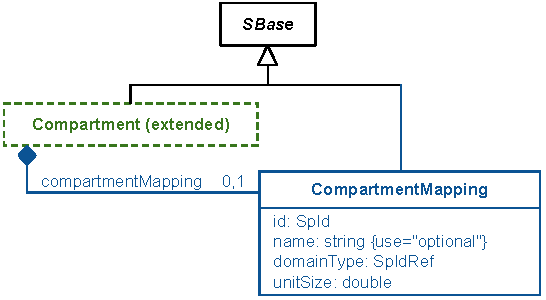
\includegraphics{figs/extended-compartment-uml}
  \caption{The definition of the extension to the \Compartment element, and the definition of the \CompartmentMapping class. The SBML core attributes of \Compartment are not displayed.}
  \label{compartment-uml}
  \label{CompartmentMapping-uml}
\end{figure}



The \Compartment element has an optional \CompartmentMapping child which indicates the \DomainType to which the \Compartment is mapped.  If there is no \CompartmentMapping for a \Compartment in a spatial model, then that \Compartment is excluded from the spatial version of the model.  In the same way, if a \DomainType is not mapped to one or more \Compartments, then the corresponding \Domains in the geometry have no assigned function.


\subsection{The \class{CompartmentMapping} class}
\label{compartmentmapping-class}
Each \Compartment in a model that defines a spatial geometry may contain an optional \CompartmentMapping. A \CompartmentMapping is defined as part of the model rather than part of the geometry so that the geometry is modular and may be readily shared between models and reused.  A \CompartmentMapping maps a \Compartment defined in the model to a \DomainType defined in the geometry such that each corresponding \DomainType is assigned the same biological and mathematical function described by the set of \Compartments that are mapped to that \DomainType. 

This mapping need not be one-to-one.  In fact, it is common to map er-lumen, er-membrane, and cytosol to the same cell interior volume or 3D \DomainType.  The \token{unitSize} attribute specifies the relative quantity of each \Compartment that is mapped to the \DomainType.

\subsubsection{The \fixttspace\tokenNC{id} and \fixttspace\tokenNC{name} attributes}
The \token{id} attribute is a mandatory attribute of type \primtype{SpId} that is used to uniquely identify a \CompartmentMapping in the model.  All identifiers of type \primtype{SpId} must be unique within the \Geometry.  The mathematical value of a \CompartmentMapping is its \token{unitSize} attribute, and can be bound to a \Parameter by using a \SpatialSymbolReference.  The optional \token{name} attribute is of type \primtype{string}, may be used to add a human-readable label to the object, and has no uniqueness requirements.

\subsubsection{The \fixttspace\tokenNC{domainType} attribute}
The mandatory \token{domainType} attribute is of type \primtype{SpIdRef} that indicates a \DomainType defined in the \Geometry element.

\subsubsection{The \fixttspace\tokenNC{unitSize} attribute}
The \token{unitSize} attribute is of type \primtype{double} and represents the relative size of the \Compartment with respect to the size of the \Domains to which they are mapped.  Thus for any infinitesimal subset of the \Domain with size S, there exists an amount of Compartment$_{\text{i}}$ of size (S*unitSize$_{\text{i}}$) for i=1..N compartments mapped to that \DomainType.  For example, a 3D \Compartment (and \DomainType) which is mapped to a 3D \DomainType has a \token{unitSize} which is a volume fraction of dimensionless unit.  The total set of all such volume fractions mapped to a particular \DomainType will typically sum to one. 

If the \token{spatialDimensions} attribute of the parent \Compartment is different than the \token{spatialDimensions} attribute of referenced \DomainType, the \token{unitSize} attribute is a conversion factor between the two.  The most common example of this would be a 2D \Compartment being mapped to a 3D \DomainType, such as an ER-membrane being mapped to a volumetric cell interior.  In this case, the \token{unitSize} is a surface-to-volume ratio.

If connected to a \Parameter via a \SpatialSymbolReference, an \InitialAssignment may override the value of the \token{unitSize} attribute.  It is theoretically possible to have this value change in time through the use of a \Rule or \Event, but some (if not all) software tools may not support this setup.  If the value is set to change, and the dimensionality of the parent \Compartment and referenced \DomainType is the same, the other \CompartmentMapping elements for the same \DomainType will typically change in concert, so that they continue to sum to one.  Also note that \Species amounts are preserved in SBML, so a changing \token{unitSize} may induce a corresponding change in any correlated \Species concentration.

Any bound \Parameter's units should be equivalent to the units of the parent \Compartment divided by the units of the referenced \DomainType. 

Here is an example of a \Compartment element extended to have spatial information:

\begin{example}
  <compartment id="Extracellular" spatialDimensions="3" constant="true">
    <spatial:compartmentMapping spatial:id="spatialExtracellular"
        spatial:domainType="Extracellular" spatial:unitSize="1"/>
  </compartment>
\end{example}



\subsection{The extended \Species object}
\label{extended-species-class}
The SBML core \Species is extended when a spatial geometry is defined in the model with the addition of a single new required boolean \val{isSpatial} attribute.  The extension to the \Species element is shown in \fig{species-uml}.
 
\begin{figure}[ht]
  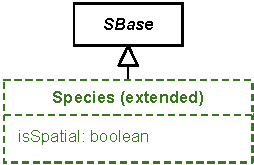
\includegraphics{figs/extended-species-uml}
  \caption{The extension to the \Species element. The attributes of \Species from \sbmlthreecore are not displayed.}
  \label{species-uml}
\end{figure}



\subsubsection{The \fixttspace\tokenNC{isSpatial} attribute}
The \token{isSpatial} attribute is of data type boolean. If it is set to true, the \Species is spatially distributed in a possibly nonhomogeneous manner within the \Domains of the same type as the mapped \DomainType. 

For continuous deterministic models (described by partial differential equations), a spatial \Species will result in a concentration field described by a partial differential equation which incorporates contributions from \Reactions, diffusion (\DiffusionCoefficient) and advection (\AdvectionCoefficient) and are subject to boundary conditions (\BoundaryCondition) and initial conditions (\InitialAssignment and \Rule).  All of these quantities can be explicit functions of the spatial coordinates as well as spatial and nonspatial \Parameters and \Species.  

For stochastic models, the \Species is represented as a collection of particles that are distributed throughout the \Domains and are subject to reactions, diffusion and advection.  Simulation algorithms either track individual particles (e.g. Particle-based methods) or use spatial discretization to track a large number of well stirred pools (e.g. Next-Subvolume Method).

The \token{compartment} of any \Species set \token{isSpatial} = \val{true} must have a child \CompartmentMapping: if it did not, its compartment would not actually be a part of the spatial model.


\subsection{The extended \Parameter object}
\label{extended-parameter-class}
When an SBML model defines a spatial geometry, the SBML core \Parameter is used to define the diffusion coefficient, transport velocity (advection) and boundary conditions for species and the coordinate components defined in the \Geometry. One \Parameter is created for each quantity, by adding a child \DiffusionCoefficient, \AdvectionCoefficient, or \BoundaryCondition.  Conversely, some elements defined in the spatial package may need to be referenced by mathematics in core constructs, or even have their value set by core constructs such as \InitialAssignment or \Rule.  These spatial elements can be semantically linked to a \Parameter by giving it a child \SpatialSymbolReference pointing to that element.

A \Parameter that has been extended for the Spatial package can have only one of the above listed objects.  For example, if a \Parameter is extended to represent the diffusion coefficient of a species, the existing attributes of the \Parameter (id, name, value, units, constant) are defined according to SBML core specifications, along with a \DiffusionCoefficient child that contains the information about the species it represents. \fig{parameter-uml} represents the extension to the \Parameter element.

\begin{figure}[ht]
  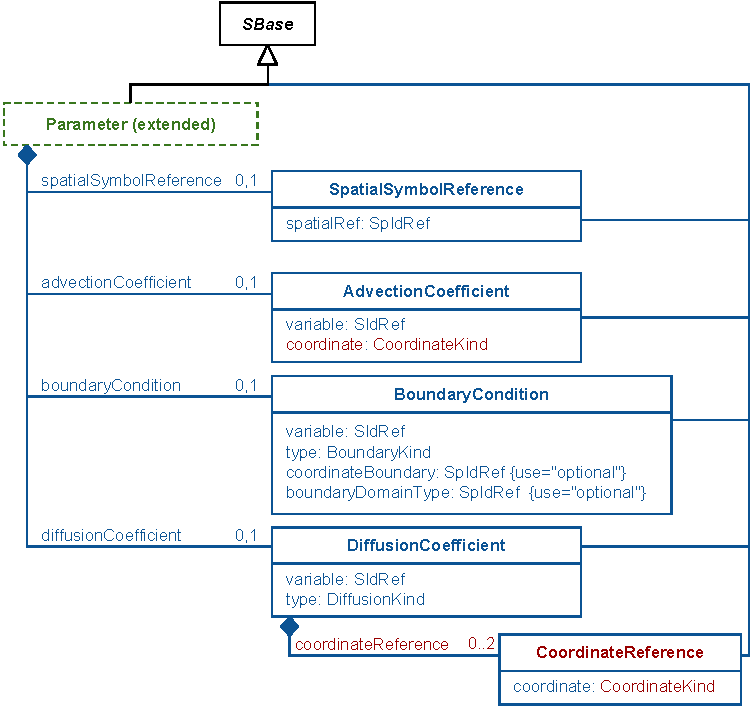
\includegraphics{figs/extended-parameter-uml}
  \caption{The \Parameter element extension for spatial package, and the definitions of the \SpatialSymbolReference, \AdvectionCoefficient, \BoundaryCondition, and \DiffusionCoefficient classes. The \sbmlthreecore attributes for \Parameter are not displayed in this figure.}
  \label{parameter-uml}
\end{figure}



\subsection{The \class{SpatialSymbolReference} class}
\label{spatialsymbolreference-class}
A \Parameter is extended with a \SpatialSymbolReference element, when a symbol from the defined spatial geometry (\token{id} of any element contained in \Geometry) is required to be used in the SBML core model. Typically, the \SpatialSymbolReference is used to represent the coordinate components defined in the \Geometry's listOfCoordinateComponents.  For example, if the \Geometry is defined in a 2-dimensional Cartesian coordinate system with X and Y defined as coordinate components, two \Parameters (one each for \CoordinateComponents X and Y) are created in the model. The value of the parameter is not required to be set. For each of these parameters, a \SpatialSymbolReference object is created.

\subsubsection{The \fixttspace\tokenNC{spatialRef} attribute}
The \token{spatialRef} attribute of \SpatialSymbolReference, is of type \primtype{SpIdRef} and refers to the \primtype{SpId} of any element defined in the \Geometry of the model.

\subsection{The \class{DiffusionCoefficient} class}
\label{diffusioncoefficient-class}
When a species in a spatial model has a diffusion rate constant, a \Parameter for this diffusion constant is created in the SBML model with a \DiffusionCoefficient child, which is used to identify the \Species whose diffusion rate the \Parameter represents. The diffusion coefficient can then be set like any other variable:  its initial value can be set using the \Parameter's \token{value} attribute or through an \InitialAssignment, and if the diffusion coefficient changes in time, this can be defined with a \Rule or \Event. If set, the units of this \Parameter should be length$^2$/time.  If left unset, the \DiffusionCoefficient will inherit the model units of length$^2$/time (typically cm$^2$s$^{-1}$ or um$^2$s$^{-1}$).


It is possible to define both diffusion and advection for the same \Species.

\subsubsection{The \fixttspace\tokenNC{variable} attribute}
The required \token{variable} attribute of \DiffusionCoefficient is of type \primtype{SIdRef} and is the \primtype{SId} of the \Species or \Parameter in the model whose diffusion coefficient is being set.

\subsubsection{The \fixttspace\tokenNC{type} and \tokenNC{coordinateReference} attributes}
The required \token{type} attribute of \DiffusionCoefficient is of type \primtype{DiffusionKind} and indicates whether the diffusion coefficient is \val{isotropic} (i.e. applies equally in all dimensions/directions), \val{anisotropic} (i.e. applies only for a single coordinate), or \val{tensor} (i.e. applies only for a particular pair of coordinates). Coefficients of type \val{isotropic} may not have any \token{coordinateReference} attributes defined, since diffusion is defined for all axes.  Coefficients of type \val{anisotropic} must define the \token{coordinateReference1} attribute and not the \token{coordinateReference2} attribute, and applies in the direction of that axis.  Coefficients of type \val{tensor} must define both the attributes \token{coordinateReference1} and \token{coordinateReference2}, defining diffusion in relation to the direction due to a gradient in the diagonal term of the diffusion tensor for the two coordinates.  In no case may \token{coordinateReference2} be defined but not \token{coordinateReference1}.

\subsubsection{\DiffusionCoefficient uniqueness}
Only one \DiffusionCoefficient may be defined per \Species per axis or pair of valid axes in the \Compartment in which it resides.  Since isotropic diffusion is defined for all axes at once, this means that if an isotropic \DiffusionCoefficient is defined for a \Species, it may have no other diffusuion coefficients.


\subsection{The \class{AdvectionCoefficient} class}
\label{advectioncoefficient-class}
The \AdvectionCoefficient is the extension to \Parameter in SBML core that is used to represent transport velocity of a species, if it exists. The transport velocity for the species is defined in a manner similar to the diffusion constant with a unit of length/time (regardless of the units of the corresponding \Species' \val{compartment} attribute).  A \Parameter is created in SBML code for the velocity with an \AdvectionCoefficient child to identify the \Species whose velocity is represented by the \Parameter; its initial value is set either through the \token{value} attribute or an \InitialAssignment.    If the advection coefficient changes in time or space, this can be modeled with a \Rule or \Event.

If defined, the units of the parent \Parameter should be in length/time; if not defined, it inherits from the model-wide units of length divided by the model-wide units of time.

It is possible to define both diffusion and advection for the same \Species.

\subsubsection{The \fixttspace\tokenNC{variable} attribute}
The \token{variable} attribute of \AdvectionCoefficient is of type \primtype{SIdRef} and is the SId of the \Species or \Parameter in the model whose advection coefficient (transport velocity) is being set.

\subsubsection{The \fixttspace\tokenNC{coordinate} attribute}
The \token{coordinate} is of type \primtype{CoordinateKind} and represents the coordinate component of the velocity. For example, if the \Geometry is defined in the Cartesian coordinate system and is 2-dimensional, the species can have velocity terms for both X and Y. If the \Parameter represents the transport velocity of the species in the X-coordinate, the \token{coordinate} attribute will take a value of \val{cartesianX}, and if it represents the velocity in the Y-coordinate, the attribute will take a value of \val{cartesianY}.  Only one \AdvectionCoefficient may be defined per \Species per valid \token{coordinate}.


\subsection{The \class{BoundaryCondition} class}
\label{boundarycondition-class}
A \Species in a spatial model that has a diffusion rate or an advection velocity needs to have specified boundary conditions. A boundary condition is either the concentration of the species or the flux density of the species at a boundary.  The boundary refers to either an internal membrane boundary or a face of the box defined by the minimum and maximum coordinates of the geometry (the geometries bounding box).

When creating a spatial SBML model, species boundary conditions are created as parameters, one for each boundary condition, by adding a child \BoundaryCondition that points to the corresponding \Species and boundary, depending on the coordinate system.

For Cartesian Geometries, there are two boundaries for every axis being modeled.  For example, in a 2D cartesian geometry for the external boundaries, there could be up to four parameters or parameter sets created for each spatial \Species whose \Compartments abut the minimum and maximums of the X and Y axes).

%For polar and cylendrical Geometries, there is one boundary for the maximum of the radius, and another boundary for the minimum of the radius if that minimum is not \val{0}.  For the azimuth, there are either two boundaries corresponding to the minimum and maximum azimuth, or no boundaries, if the minimum is 0$^\circ$, and the maximum is 360$^\circ$.  In cylendrical geometry, there will be two boundaries for the minumum and maximum height.

%For spherical Geometries, there will again be one boundary for the maximum of the radius, and another boundary for the minumum of the radius if that minimum is not \val{0}.  For the spherical azimuth and elevation, there will be either two boundaries each corresponding to the minimum and maximum values, or no boundaries, for each minimum 0$^\circ$ and maximum 360$^\circ$ pair.

For internal boundaries, one may either define a \BoundaryCondition for a \Species at that boundary, or one may define one or more transport reactions that describe how the physical entities that \Species represent are moved (or converted) from one side of the boundary to the other.  One may not define both a \BoundaryCondition and a \Reaction that describes the same phenomenon, as this would result in the equivalent of an overdetermined system, not dissimilar from the reason that the change in a \Species may not be defined by both a \Reaction and a \RateRule.  A \Species set \token{boundaryCondition} = \val{true} may have a defined \BoundaryCondition and also appear in a transport \Reaction, but its change in time and space will only be determined by the \BoundaryCondition.

If neither a \BoundaryCondition nor a \Reaction is defined for a particular \Species/boundary pair, the flux of that \Species at that boundary is zero.

The \Parameter's value is set either through the \token{value} attribute or an \InitialAssignment.  If the boundary condition changes in time, it can be set with a \Rule or \Event.  If set, the \Parameter unit must be equal to the appropriate unit for its \token{type} (see below).  Only one \BoundaryCondition may be defined per \Species per boundary (regardless of type).


\subsubsection{The \fixttspace\tokenNC{variable} attribute}
The \token{variable} attribute of \BoundaryCondition is of type \primtype{SIdRef} and is the SId of the \Species or \Parameter in the model whose boundary condition is being set.

\subsubsection{The \fixttspace\tokenNC{type} attribute}
The \token{type} attribute is of type \primtype{BoundaryConditionKind} and indicates the type of boundary condition. The boundary condition types come in three groups: for Neumann boundaries, \val{Neumann} (the inward normal flux) is used.  For Dirichlet boundaries, \val{Dirichlet} (the value) is used.  For Robin boundaries, three different Parameters must be defined, with \BoundaryCondition elements of type \val{Robin\_inwardNormalGradientCoefficient}, \val{Robin\_valueCoefficient}, and \val{Robin\_sum}.

The unit of the boundary condition is determined by the type, and the unit for density and velocity.  For \val{Dirichlet}, the unit would be the unit of concentration.  For \val{Neumann}, the unit would be concentration*length/time.  For Robin boundaries, for a variable \val{u} with an inward pointing normal vector \val{n}, Robin value coefficient \val{a}, Robin inward normal gradient coefficient \val{b}, and Robin sum \val{g}, the condition is defined by the equation \val{a*u + b*inner\_product(grad(u),n) = g}, with appropriate units.  The suggested set of units that satisfy this condition is to have units of nondimensional for \val{a}, 1/length for \val{b}, and the same units as the referenced \token{variable} for \val{c}.

\subsubsection{The \fixttspace\tokenNC{coordinateBoundary} attribute}
The \token{coordinateBoundary} attribute is of type \primtype{SpIdRef} and refers to the \primtype{SpId} of either the \token{boundaryMin} or the \token{boundaryMax} object of the \CoordinateComponent defined in \Geometry. This \primtype{SpId} indicates the boundary condition (minimum or maximum) in the \CoordinateComponent. A \Parameter that is extended with a \BoundaryCondition object can only define the \token{coordinateBoundary} attribute or the \token{boundaryDomainType} attribute, but not both.

\subsubsection{The \fixttspace\tokenNC{boundaryDomainType} attribute}
The \token{boundaryDomainType} attribute is of type \primtype{SpIdRef} and refers to the \primtype{SpId} of the \DomainType of the location of the species whose boundary condition is being defined. A \Parameter that is extended with a \BoundaryCondition object can only define the \token{coordinateBoundary} attribute or the \token{boundaryDomainType} attribute, but not both. 


\subsection{Extended \Parameter examples}

As an example, here are four examples of parameters that have been extended with spatial information.  These four parameters are extended with the four different possible spatial extensions: the \SpatialSymbolReference to allow the model to refer to the spatial id \val{x} as the SBML core id \val{x}; a \BoundaryCondition to define the boundary condition for \val{s1\_nuc} to be zero; a \DiffusionCoefficient to define the diffusion coefficient for \val{s1\_nuc} to be \val{0.1}; and an \AdvectionCoefficient to define the advection coefficient for \val{s2\_nuc} to be \val{0.13}.

\begin{example}
  <listOfParameters>
    <parameter id="x" constant="false">
      <spatial:spatialSymbolReference spatial:spatialRef="x"/>
    </parameter>
    <parameter id="s1_nuc_BC_Xm" value="0" constant="true">
      <spatial:boundaryCondition spatial:variable="s1_nuc" spatial:type="Dirichlet"
                                 spatial:coordinateBoundary="Xmin"/>
    </parameter>
    <parameter id="s1_nuc_diff" value="0.1" constant="true">
      <spatial:diffusionCoefficient spatial:variable="s1_nuc" spatial:type="isotropic"/>
    </parameter>
    <parameter id="s2_nuc_advec" value="0.13" constant="true">
      <spatial:advectionCoefficient spatial:variable="s2_nuc" spatial:coordinate="cartesianX"/>
    </parameter>
  </listOfParameters>
\end{example}

\subsection{The extended \Reaction object}
\label{extended-reaction-class}
The SBML core \Reaction is extended when a spatial geometry is defined in the model with the addition of a single new required boolean \token{isLocal} attribute. \fig{reaction-uml} displays the definition of the extension of the \Reaction element.
 
\begin{figure}[ht]
  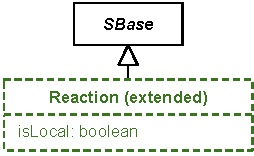
\includegraphics{figs/extended-reaction-uml}
  \caption{The extension to the \Reaction element. The \sbmlthreecore atrributes and children for \Reaction are not displayed in the figure.}
  \label{reaction-uml}
\end{figure}

\subsubsection{The \fixttspace\tokenNC{isLocal} attribute}
The \token{isLocal} attribute for a \Reaction is of type \primtype{Boolean}. The attribute is set to true if the reaction is to be considered a local description of the reaction in terms of concentration/time defined at each point in space rather than substance/time over an entire \Compartment or "pool".  Note that this means that the units of the \KineticLaw are different depending on whether the \Reaction is local or not.

If a \Reaction is defined to be a local (having an \token{isLocal} value of \val{true}), the value of the \token{compartment} attribute of the \Reaction must be defined.  This is because the interpretation of the \Reaction is very different if the reaction takes place at the boundary of the \Compartment of the \Species (where the reaction rate units are flux densities) than if it takes place within the interior of that \Compartment (where the reaction rate units are concentration/time define throughout the volume).  The first will give you gradients in the solution, while the other will not.

If the referenced \Species come from multiple compartments, the \token{compartment} of the \Reaction must be a \Compartment that makes physical sense for the individual \Species to meet.

\subsection{The \class{Geometry} class}
\label{geometry-class}
\label{listofcoordinatecomponents-class}
\label{listofdomaintypes-class}
\label{listofdomains-class}
\label{listofadjacentdomains-class}
\label{listofgeometrydefinitions-class}
\label{listofsampledfields-class}

A single geometry must be defined within the model if the spatial extension is to be used. \fig{Geometry-uml} shows the definition of the \Geometry element.
 
\begin{figure}[ht]
  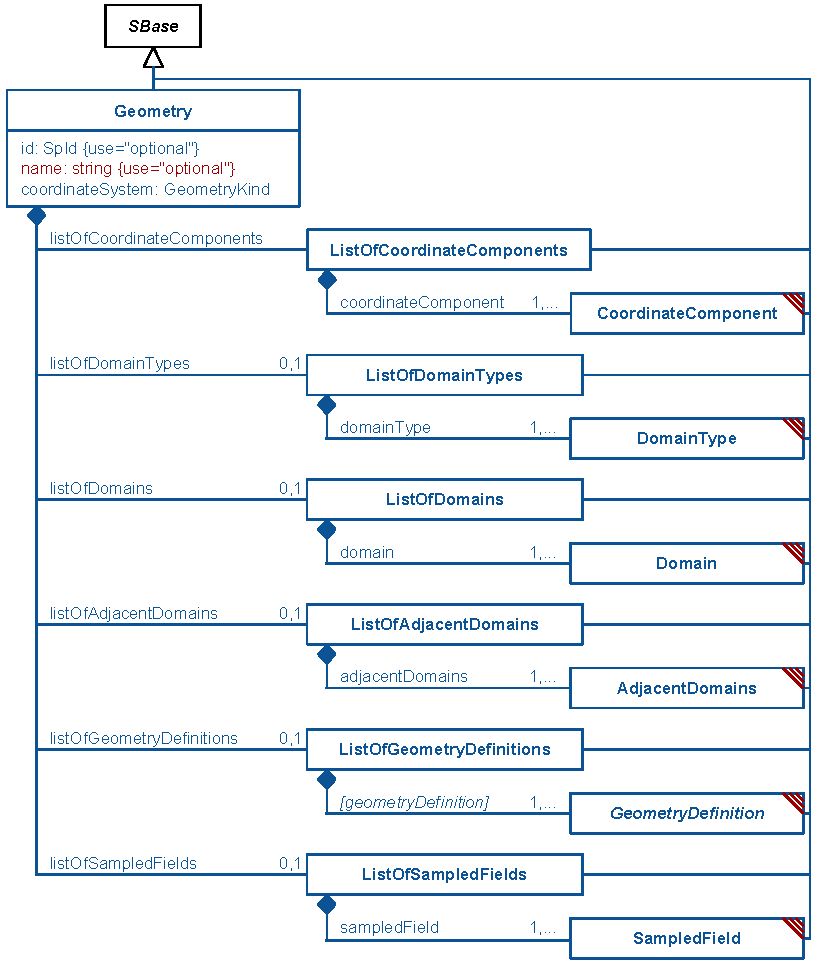
\includegraphics{figs/Geometry-uml}
  \caption{The definition of the \Geometry, \ListOfCoordinateComponents, \ListOfDomainTypes, \ListOfDomains, \ListOfAdjacentDomains, \ListOfGeometryDefinitions, and \ListOfSampledFields classes from the Spatial package.  The various children of the ListOf- classes are defined in their own sections.}
  \label{Geometry-uml}
  \label{ListOfCoordinateComponents-uml}
  \label{ListOfDomainTypes-uml}
  \label{ListOfDomains-uml}
  \label{ListOfAdjacentDomains-uml}
  \label{ListOfGeometryDefinitions-uml}
  \label{ListOfSampledFields-uml}
\end{figure}

\subsubsection{The \fixttspace\tokenNC{id} and \fixttspace\tokenNC{name} attributes}
The \token{id} attribute is of type \primtype{SpId}, uniquely identifies the \Geometry element, and is optional.  It has no mathematical meaning, and cannot be connected to a \Parameter via a \SpatialSymbolReference element.  The optional \token{name} attribute is of type \primtype{string}, may be used to add a human-readable label to the object, and has no uniqueness requirements.

\subsubsection{The \fixttspace\tokenNC{coordinateSystem} attribute}
The \token{coordinateSystem} attribute is a required attribute and is of type \primtype{GeometryKind}. It represents the coordinate system used by the \Geometry.  A value of  \val{cartesian} indicates that the geometry is a cartesian coordinate system, with the coordinate components corresponding to the x, y, and z components of that system (which could be 1-, 2-, or 3-dimensional).  This is the only coordinate system defined in this version of the specification--in the future, if necessary, \val{cylendrical}, \val{spherical}, and \val{polar} may be added as possibilities, along with n-dimensional cartesian modeling, should there be interest in the modeling community to exchange these types of models.

%A value of \val{cylindrical} indicates that the geometry is a three-dimensional cylendrical coordinate system, with coordinate components corresponding to radial distance, azimuth angle, and axial position.  A value of \val{spherical} indicates that the geometry is a three-dimensional spherical coordinate system, with coordinate components corresponding to radial distance, polar angle, and azimuth angle.  A value of \val{polar} indicates that the geometry is a two-dimensional polar coordinate system, with coordinate components corresponding to radial distance and angle (the two-dimensional equivalent of the cylendrical coordinate system).

\subsubsection{The listOf container classes}
The \Geometry has listOfCoordinateComponents, listOfDomainTypes, listOfDomains, listOfAdjacentDomains, listOfGeometryDefinitions, and listOfSampledFields that help define the geometry.  The \ListOfCoordinateComponents is a list of \CoordinateComponent objects, the \ListOfDomainTypes is a list of \DomainType objects, the \ListOfDomains is a list of \Domain objects, \ListOfAdjacentDomains is a list of \AdjacentDomains objects, the \ListOfGeometryDefinitions is a list of alternative \GeometryDefinitions (\ParametricGeometry, \CSGeometry, \SampledFieldGeometry, \AnalyticGeometry, and \MixedGeometry), and the \ListOfSampledFields is a list of \SampledField objects.  Of these, only the \ListOfCoordinateComponents is required, but, if present, none of them may be empty.

Note that the children of the \ListOfGeometryDefinitions object are not called \token{geometryDefinition} but rather take the name of the derived class, decapitalized.  Thus, they may be called \token{analyticGeometry}, \token{csGeometry}, \token{parametricGeometry}, \token{sampledFieldGeometry}, or \token{mixedGeometry}.

The \ListOfCoordinateComponents is unique in that it defines the dimensions of the \Geometry.  Thus, every \Geometry must have a child \ListOfCoordinateComponents with exactly one, two, or three children.  When there is one child, it must be of type \token{cartesianX}; when there are two, they must be of type \token{cartesianX} and \token{cartesianY}, and when there are three, they must be of types \token{cartesianX}, \token{cartesianY}, and \token{cartesianZ}.


\subsection{The \class{CoordinateComponent} class}
\label{coordinatecomponent-class}
A \CoordinateComponent object explicitly defines a coordinate component of the coordinate axes and gives them names, units, and formally associates them with a coordinate system. The \CoordinateComponent also defines the minimum and maximum values of the coordinate axis it represents. The definition of \CoordinateComponent is shown in \fig{CoordinateComponent-uml}.
 
\begin{figure}[ht]
  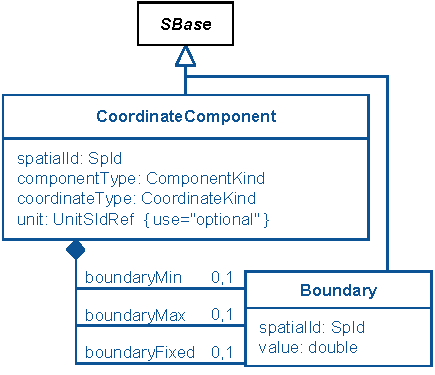
\includegraphics{figs/CoordinateComponent-uml}
  \caption{The \CoordinateComponent and \Boundary object definitions. One or more instances of \CoordinateComponent objects in a \ListOfCoordinateComponents can be present in \Geometry.}
  \label{CoordinateComponent-uml}
\end{figure}


\subsubsection{The \fixttspace\tokenNC{id} and \fixttspace\tokenNC{name} attributes}
A \CoordinateComponent is identified with the \token{id} attribute which is of type \primtype{SpId}.  The mathematical value of a \CoordinateComponent is its coordinate value \token{unitSize} attribute, and can be bound to a \Parameter by using a \SpatialSymbolReference.  The optional \token{name} attribute is of type \primtype{string}, may be used to add a human-readable label to the object, and has no uniqueness requirements.
 
Because a \CoordinateComponent represents an entire axis, it is not appropriate, should it be connected to a \Parameter via a \SpatialSymbolReference, for that \Parameter to be set via an \InitialAssignment or \Rule.  Rather, it is treated like the SBML core \token{csymbol} \val{time}, and can be used as an independent variable in other calculations.

\subsubsection{The \fixttspace\tokenNC{type} attribute}
The \token{type} attibute of type \primtype{CoordinateKind} represents the type of the coordinate component, and may take one of a subset of all possible \primtype{CoordinateKind} values depending on its parent \Geometry, as defined in \tab{CoordinateComponent-Geometry-relation}.
%For all \primtype{GeometryKind} values except \val{cartesian}, exactly one \CoordinateComponent must exist with each of the allowed \primtype{CoordinateKind} values:  in other words, a \val{cylendrical} \Geometry must have exactly three \CoordinateComponent children, each one having a different allowed value for its \token{type} attribute.
For Cartesian geometries, one-dimensional geometries must be defined by having a single \val{cartesianX} \CoordinateComponent; two-dimensional geometries must be defined by having exactly two \CoordinateComponent children with \token{type} values of \val{cartesianX} and \val{cartesianY}, and three-dimensional geometries must be defined by having exactly three \CoordinateComponent children with \token{type} values of \val{cartesianX}, \val{cartesianY}, and \val{cartesianZ}.  No \Geometry may have two \CoordinateComponent children with the same \token{type}.

\begin{table}[thb]
  \begin{edtable}{tabular}{>{\centering\arraybackslash}m{0.9in} >{\centering\arraybackslash}m{0.7in} >{\raggedright\arraybackslash}m{4.4in}}
  %\begin{edtable}{tabular}{p{0.9in}p{0.7in}p{4.4in}}
    \toprule
    \textbf{GeometryKind} & \textbf{Dimensions} & \textbf{CoordinateKinds} \\
    \midrule
    \token{cartesian}   & 1 & \val{cartesianX} (\token{coord1})\\
    \token{cartesian}   & 2 & \val{cartesianX} (\token{coord1}) and \val{cartesianY} (\token{coord2})\\
    \token{cartesian}   & 3 & \val{cartesianX} (\token{coord1}), \val{cartesianY} (\token{coord2}), and \val{cartesianZ} (\token{coord3})\\
 %   \token{cylendrical} & 3 & \val{cylindricalRadius} (\token{coord1}), \val{cylindricalAzimuth} (\token{coord2}), and \val{cylindricalHeight} (\token{coord3})\\
 %   \token{polar}       & 2 & \val{polarRadius} (\token{coord1}) and \val{polarAzimuth} (\token{coord2})\\
 %   \token{spherical}   & 3 & \val{sphericalRadius} (\token{coord1}), \val{sphericalAzimuth} (\token{coord2}), and \val{sphericalElevation} (\token{coord3})\\
    \bottomrule
  \end{edtable}
  \caption{Correspondance between the \token{type} of a \Geometry and the possible \token{type}s of its child \CoordinateComponent elements.  Also noted is the corresponding attribute (\token{coord1}, \token{coord2}, or \token{coord3}) corresponding to each axis when defining \InteriorPoint elements (see \sec{interiorpoint-class}).} 
  \label{CoordinateComponent-Geometry-relation}
\end{table}



%\subsubsection{The \fixttspace\tokenNC{coordinateType} attribute}
%The \token{coordinateType} attribute, of type \primtype{CoordinateKind}, represents whether the axis being defined is normal (\val{normal}), or whether it represents a dimension that does not need to be modeled explicitly in any performed calculations, whether due to symmery, where the modeled element exists in the given dimension, but is assumed to be the same for all values along that axis (\val{symmetrical}), or due to being constrained to a single value along that axis (\val{fixed}).

%\CoordinateComponent elements of coordinateType \val{normal} must have a \token{boundaryMin} and \token{boundaryMax} child.  \CoordinateComponent elements of coordinateType \val{symmetrical} may have a \token{boundaryMin} and \token{boundaryMax} children for visualization purposes, but they are optional.  \CoordinateComponent elements of coordinateType \val{fixed} must have a single \token{boundaryFixed} child.


\subsubsection{The \fixttspace\tokenNC{unit} attribute}
The unit of a \CoordinateComponent is represented by the \token{unit} attribute, of type \primtype{UnitSIdRef}.  If not specified, the unit of a \CoordinateComponent inherits from the \token{lengthUnits} attribute of the \Model object, and if that in turn is not specified, the \CoordinateComponent units cannot be determined.
%Many coordinates may have different units from the \token{lengthUnits} of the \Model, since this is a distance metric and not always the same as the unit of each individual coordinate.  For example, in Polar coordinates, the coordinate component 'theta' may be described in radians while component 'rho' may be in microns.  


\subsection{The \class{Boundary} class}
\label{boundary-class}
The minimum and the maximum for a \CoordinateComponent represent the bounds in each coordinate.  For example, for three dimensional Cartesian coordinate system with x, y, and z coordinates, the minimum and maximum limits for each coordinates define planes orthogonal to each coordinate axis and passing through the minimum or maximum.  If max-min is the same for each x,y,z then the bounds on the geometry is a cube.  The \Boundary class interacts with the \BoundaryCondition class, allowing modelers to define how model elements behave at the boundary of the model.  For species defined within volumes adjacent to these surfaces, \BoundaryCondition elements must be introduced.

%{\color{red} Lucian: \notice Just a note to coordinate the text here to sync with the text in the \BoundaryCondition class, if that changes.  }

The minimum limit of a \CoordinateComponent is represented by the \token{boundaryMin} object and the maximum limit is represented by the \token{boundaryMax} object, and apply to \CoordinateComponent elements.
%of coordinateType \val{normal} and \val{symmetrical} (and are optional in the latter case only).
Both are \Boundary objects, and have the following attributes:

%For \CoordinateComponent elements of coordinateType \val{fixed}, a single \token{boundaryFixed} object defines the value at which the coordinate component is fixed.  

\subsubsection{The \fixttspace\tokenNC{id} and \fixttspace\tokenNC{name} attributes}
The \token{id} attribute of the \Boundary object identifies the object.  The attribute is required and is of type \primtype{SpId}. This attribute is used when specifying the \BoundaryCondition for a species as an extension of an SBML core \Parameter.  The mathematical value of a \Boundary is its \token{value} attribute, and can be bound to a \Parameter by using a \SpatialSymbolReference.  The units are the same as its parent \CoordinateComponent, and are not set separately.  The optional \token{name} attribute is of type \primtype{string}, may be used to add a human-readable label to the object, and has no uniqueness requirements.

\subsubsection{The \fixttspace\tokenNC{value} attribute}
The \token{value} attribute is of type \primtype{double}. In a \token{boundaryMin} object, it represents the minimum limit of the \CoordinateComponent.  In a \token{boundaryMax} object, it represents the maximum limit of the \CoordinateComponent.

%In a \token{boundaryFixed} object, it represents the fixed level of the \CoordinateComponent.

If connected to a \Parameter via a \SpatialSymbolReference, this \token{value} may be overridden by an \InitialAssignment.  However, the \Parameter must be set \token{constant}=\val{true}, because it may not change over the course of the simulation.


\subsubsection{A \CoordinateComponent example}
In this example, a \CoordinateComponent is used to define an X axis that goes from 0 to 10 um.

\begin{example}
  <spatial:coordinateComponent spatial:id="x" spatial:type="cartesianX" spatial:unit="um">
    <spatial:boundaryMin spatial:id="Xmin" spatial:value="0"/>
    <spatial:boundaryMax spatial:id="Xmax" spatial:value="10"/>
  </spatial:coordinateComponent>
\end{example}


\subsection{The \class{DomainType} class}
\label{domaintype-class}
A \DomainType is a class of domains that are identified as being anatomically and physiologically similar.  For example, a \DomainType "cytosol" may be defined in a \Geometry as identifying the structure and function of the cell interior.  If there is one cell, then there is one domain, if there are multiple cells, then there are multiple disjoint domains ("cytosol1","cytosol2", etc.) identified with the \DomainType "cytosol".  \CompartmentMappings, defined as an extension to an SBML core \Compartment, map compartments to domain types such that each corresponding domain is assigned the same biological and mathematical function. \fig{DomainType-uml} shows the \DomainType object.

Each SBML \Compartment maps to a single \DomainType, meaning that the initial condition of each \Species in each \Compartment will be the same across all \Domains that map to a given \DomainType.  If those \Species are spatially distributed, they will subsequently evolve independently from each other.  However, if modeling two \Domains that are similar but whose \Species have different initial conditions, those \Domains should be modeled as separate \DomainTypes.

\begin{figure}[ht]
  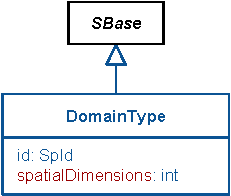
\includegraphics{figs/DomainType-uml}
  \caption{The definition of the \DomainType class. One or more instances of \DomainType in a \ListOfDomainTypes instance can be present in a \Geometry object.}
  \label{DomainType-uml}
\end{figure}

\subsubsection{The \fixttspace\tokenNC{id} and \fixttspace\tokenNC{name} attributes}
Each \DomainType is identified with a \token{id} of type \primtype{SpId}.  The mathematical value of a \CompartmentMapping is the sum of the sizes of all domains associated with this \DomainType, and can be bound to a \Parameter by using a \SpatialSymbolReference.  The optional \token{name} attribute is of type \primtype{string}, may be used to add a human-readable label to the object, and has no uniqueness requirements.

As a derived quantity, if connected to a \Parameter via a \SpatialSymbolReference, this value may \emph{not} be overridden by an \InitialAssignment, nor by the use of a \Rule or \Event.  Its value is always connected to the size of its component \Domains instead.  The units of a \DomainType are the units of the corresponding base units of the SBML \Model for length (for one-dimensional domains), area (for two-dimensional domains), or volume (for three-dimensional domains).  It is required to define the corresponding base units for every \DomainType in the \Model.

\subsubsection{The \fixttspace\tokenNC{spatialDimensions} attribute}
The \token{spatialDimensions} attribute of the \DomainType is of type \primtype{int} and can take on a value of 0, 1, 2, or 3. The spatial dimension is specified for a \DomainType, rather than being repeated for each \Domain that is represented by the \DomainType.

If the \token{spatialDimensions} attribute of a \DomainType is a lower dimensionality than the \Geometry to which it refers (via the \Domain), it is considered to describe the surface of that \Geometry in the 3D case, or the perimeter of that \Geometry in the 2D case.  Since there is no defined perimeter of a 3D object, it is illegal to have a \DomainType with a \token{spatialDimensions} of \val{1} where the corresponding \Geometry is three-dimensional.


\subsection{The \class{Domain} class}
\label{domain-class}
\label{listofinteriorpoints-class}
\Domains represent contiguous regions identified by the same \DomainType.  One, two and three dimensional domains are contiguous linear regions, surface regions, and volume regions (respectively), bounded by the limits of the coordinate system (e.g. min/max of x,y,z) and adjacent domains corresponding to different domain types.  \Domain is shown in \fig{Domain-uml}.
 
\begin{figure}[ht]
  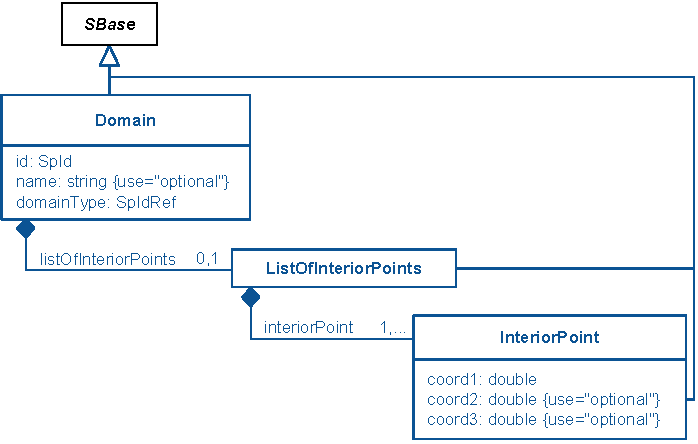
\includegraphics{figs/Domain-uml}
  \caption{The definition of the \Domain, \ListOfInteriorPoints, and \InteriorPoint classes.  A \ListOfDomains instance in \Geometry can contain one or more \Domain object instances.}
  \label{Domain-uml}
  \label{InteriorPoint-uml}
  \label{ListOfInteriorPoints-uml}
\end{figure}

\subsubsection{The \fixttspace\tokenNC{id} and \fixttspace\tokenNC{name} attributes}
A \Domain is identified with an \token{id} attribute of type \primtype{SpId}.  This \token{id} may be used within a \SpatialSymbolReference object that is extended from an SBML core \Parameter and can be used in an expression.  The mathematical value of a \Domain is the absolute size of that domain as used by the simulator (the meshed size), and can be bound to a \Parameter by using a \SpatialSymbolReference.  The optional \token{name} attribute is of type \primtype{string}, may be used to add a human-readable label to the object, and has no uniqueness requirements.

As a derived quantity, if connected to a \Parameter via a \SpatialSymbolReference, this value may \emph{not} be overridden by an \InitialAssignment, nor by the use of a \Rule or \Event.  Its value is always connected to the size of the corresponding \Geometry instead.  The units of the \Domain are the same as the units of the corresponding \DomainType.

\subsubsection{The \fixttspace\tokenNC{domainType} attribute}
The \token{domainTpe} attribute refers to the \primtype{SpId} of the \DomainType that describes the anatomy and physiology of this domain. The attribute is of type \primtype{SpIdRef}. It is through this association that compartments, and hence the whole SBML model, gets mapped to the individual domains. 


\subsection{The \class{InteriorPoint} class}
\label{interiorpoint-class}
Each \Domain can contain a \ListOfInteriorPoints. The list of spatial points for a domain is interior to that domain.  This list is optional for a \Domain if it is the only \Domain defined for its \DomainType, but is required otherwise.

For those geometric descriptions that can describe multiple disjoint domains belonging to the same \token{domainType}, these interior points allow unambiguous identification of each domain.  Formally, a single point would suffice, but in practice some tools (e.g. Smoldyn) require multiple points to handle non-convex volumes bounded by explicit surfaces.  For discontinuous surfaces with the same \token{domainType}, the interior point identifies which domain is associated with which surface patch defined in the geometry definition.

Each \InteriorPoint has three attributes: \token{coord1}, \token{coord2}, and \token{coord3}. 

\subsubsection{The \fixttspace\tokenNC{coord1}, \tokenNC{coord2}, and \tokenNC{coord3} attributes}
An InteriorPoint element represents a single point within the defined coordinate system and should be in the interior of the domain that contains it. It has three attributes, \token{coord1}, \token{coord2}, and \token{coord3}, of type \primtype{double}, representing the position along each of the up to three coordinate axes defined by the \CoordinateComponents (with \token{type} \val{cartesianX}, \val{cartesianY}, and \val{cartesianZ}, respectively, for each \token{coord\_} attribute; see \tab{CoordinateComponent-Geometry-relation}).

Each \InteriorPoint must define the same number of attributes as there are dimensions of the corresponding \Geometry to which it belongs.

In the case of surfaces, interior points are sometimes required to make unambiguous identification of multiple surfaces (e.g multiple plasma membranes for multiple cells present in a geometry).  Due to roundoff error and finite word lengths, it is difficult to find a three dimensional point that lies on a surface.  In this case, the distance from the surface will be used to provide unambiguous identification.


\subsection{The \class{AdjacentDomains} class}
\label{adjacentdomains-class}
\AdjacentDomains (or domain adjacencies) captures the topological relationships within the \Geometry.  Consider that the \Domains are nodes in a graph. The \AdjacentDomains objects are the edges that specify the spatial connectivity of these nodes.  Armed with the topology and the domain sizes, one can readily perform a compartmental approximation.  \fig{AdjacentDomains-uml} shows the definition of the \AdjacentDomains object.

\begin{figure}[ht]
  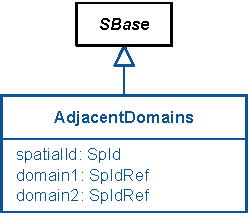
\includegraphics{figs/AdjacentDomains-uml}
  \caption{The definition of the \AdjacentDomains class. \Geometry can contain one instance of \ListOfAdjacentDomains that can have one or more instances of \AdjacentDomains objects.}
  \label{AdjacentDomains-uml}
\end{figure}

\subsubsection{The \fixttspace\tokenNC{id} and \fixttspace\tokenNC{name} attributes}
This attribute identifies an \AdjacentDomains object. The attribute is of type \primtype{SpId}.  It has no mathematical meaning, and cannot be connected to a \Parameter via a \SpatialSymbolReference element.  The optional \token{name} attribute is of type \primtype{string}, may be used to add a human-readable label to the object, and has no uniqueness requirements.

\subsubsection{The \fixttspace\tokenNC{domain1} and \tokenNC{domain2} attributes}
The \token{domain1} and \token{domain2} attributes, of type \primtype{SpIdRef}, are required attributes. They are the \primtype{SpId}'s of two domains that touch each other (spatially adjacent).  These are typically surface-volume contacts.

\subsection{Domain example}
\label{domain-example}
The following is an example of a set of \Domain, \DomainType, and \AdjacentDomains objects.

\begin{example}
  <spatial:listOfDomainTypes>
    <spatial:domainType spatial:id="Cytosol" spatial:spatialDimensions="3"/>
    <spatial:domainType spatial:id="Nucleus" spatial:spatialDimensions="3"/>
  </spatial:listOfDomainTypes>
  <spatial:listOfDomains>
    <spatial:domain spatial:id="Cytosol0" spatial:domainType="Cytosol">
      <spatial:listOfInteriorPoints>
        <spatial:interiorPoint spatial:coord1="2.4" spatial:coord2="2.4" spatial:coord3="0.5"/>
      </spatial:listOfInteriorPoints>
    </spatial:domain>
    <spatial:domain spatial:id="Nucleus0" spatial:domainType="Nucleus">
      <spatial:listOfInteriorPoints>
        <spatial:interiorPoint spatial:coord1="4.8" spatial:coord2="4.8" spatial:coord3="0.5"/>
      </spatial:listOfInteriorPoints>
    </spatial:domain>
  </spatial:listOfDomains>
  <spatial:listOfAdjacentDomains>
    <spatial:adjacentDomains spatial:domain1="Cytosol0" spatial:domain2="Nucleus0"
                             spatial:id="Nucleus_Cytosol"/>
  </spatial:listOfAdjacentDomains>
\end{example}


\subsection{The \class{GeometryDefinition} class}
\label{geometrydefinition-class}
A \Geometry can specify a list of \GeometryDefinitions. The \GeometryDefinition is an abstract class that is the general term for the container which defines the concrete geometric constructs represented by the \Geometry. Four types of \GeometryDefinitions have been identified - \AnalyticGeometry, \SampledFieldGeometry, \ParametricGeometry, \CSGeometry (Constructed Solid Geometry) - and are elaborated in the following sections. The definition of the \GeometryDefinition element is displayed in \fig{GeometryDefinition-uml}.  The spatial dimension of the \GeometryDefinition must match the \token{spatialDimensions} of the \DomainType defined for the associated \Domain.

\begin{figure}[ht]
  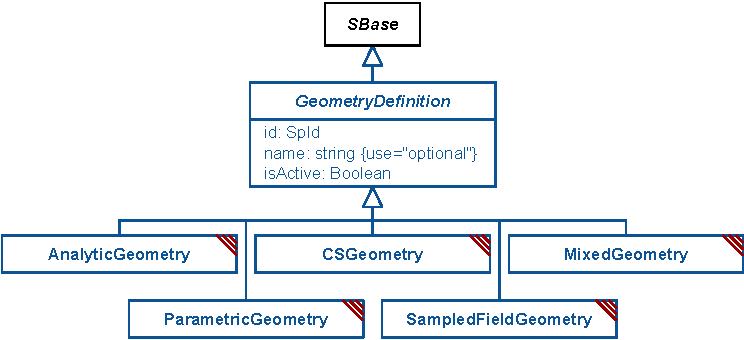
\includegraphics{figs/GeometryDefinition-uml}
  \caption{The \GeometryDefinition element. \Geometry contains one instance of listOfGeometryDefinitions that can contain one or more instances of \GeometryDefinition (one of \AnalyticGeometry, \SampledFieldGeometry, \CSGeometry, \ParametricGeometry, or \MixedGeometry, defined below).}
  \label{GeometryDefinition-uml}
\end{figure}

\subsubsection{The \fixttspace\tokenNC{id} and \fixttspace\tokenNC{name} attributes}
The \token{id} attribute is common to all the \GeometryDefinition types and is used to uniquely identify the \GeometryDefinition. The attribute is of type \primtype{SpId}.  It has no mathematical meaning, and cannot be connected to a \Parameter via a \SpatialSymbolReference element.  The optional \token{name} attribute is of type \primtype{string}, may be used to add a human-readable label to the object, and has no uniqueness requirements.

\subsubsection{The \fixttspace\tokenNC{isActive} attribute}
The \token{isActive} attribute that is common to all the \GeometryDefinition types is used to identify the \GeometryDefinition that is considered the active \GeometryDefinition for the document.  When multiple \GeometryDefinition elements define the same underlying geometry, each may set their \token{isActive} attribute to \val{true}.  At least one \GeometryDefinition in a \Model must have an \token{isActive} attribute of \val{true}, and any other \GeometryDefinition that does not describe that same underlying physical geometry must have an \token{isActive} value of \val{false}.

\subsection{The \class{AnalyticGeometry} class}
\label{analyticgeometry-class}
\label{listofanalyticvolumes-class}
The \AnalyticGeometry is a class of \GeometryDefinition where the geometry of each domain is defined by an analytic expression. An \AnalyticGeometry is defined as a collection of \AnalyticVolumes, one \AnalyticVolume for each volumetric domain in the geometry. In this representation, the surfaces are treated as the boundaries between dissimilar \AnalyticVolumes. The \AnalyticGeometry object contains a \ListOfAnalyticVolumes. \fig{AnalyticGeometry-uml} shows the definition of the \AnalyticGeometry object.

\begin{figure}[ht]
  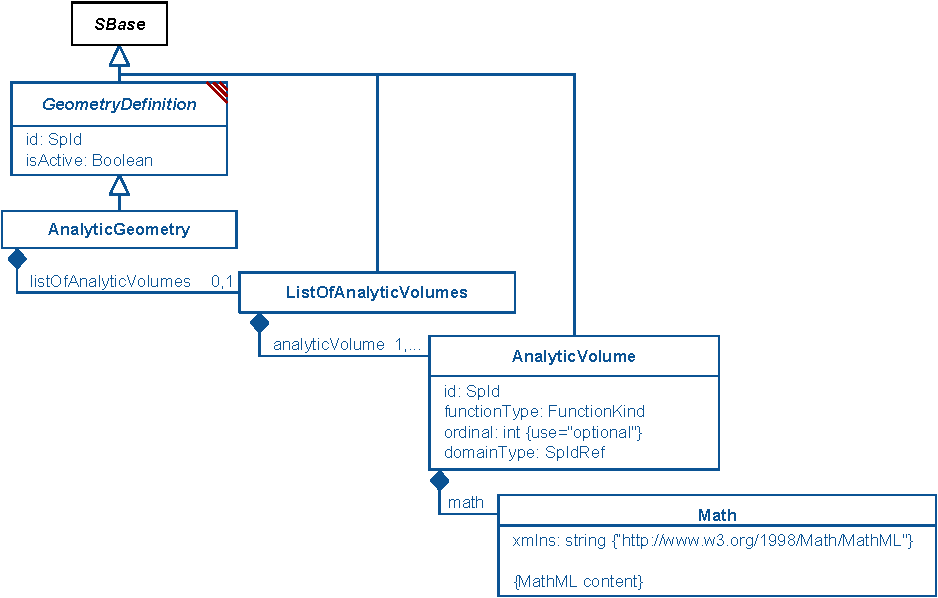
\includegraphics{figs/AnalyticGeometry-uml}
  \caption{The definition of the \AnalyticGeometry, \ListOfAnalyticVolumes, and \AnalyticVolume classes.}
  \label{AnalyticGeometry-uml}
  \label{ListOfAnalyticVolumes-uml}
  \label{AnalyticVolume-uml}
\end{figure}


\subsection{The \class{AnalyticVolume} class}
\label{analyticvolume-class}
The \AnalyticVolume is used to specify the analytic expression of a volumetric (3-dimensional) domain. The analytic expression for the \AnalyticVolume is defined in the Math element.

\subsubsection{The \fixttspace\tokenNC{id} and \fixttspace\tokenNC{name} attributes}
The \token{id} attribute uniquely identifies the \AnalyticVolume. The attribute is required and is of type \primtype{SpId}.  It has no mathematical meaning, and cannot be connected to a \Parameter via a \SpatialSymbolReference element.  The optional \token{name} attribute is of type \primtype{string}, may be used to add a human-readable label to the object, and has no uniqueness requirements.

\subsubsection{The \fixttspace\tokenNC{functionType} attribute}
The \token{functionType} attribute is of type \primtype{FunctionKind} and is currently limited to just \val{layered} (a possibility for future versions of the specification is to allow the value \val{R-function}).  A \val{layered} function type implies that the Math child element contains an inequality in the spatial dimensions (e.g. x,y,z) such that evaluation to \val{true} indicates that the point (x,y,z) is within that shape, and "false" indicates that it is not covered by that shape.
%The \val{R-function} \token{functionType} indicates that the shape is represented by a real-valued function whose sign indicates coverage by the shape.

%{\color{red} Lucian: \notice If you want to rename 'layered', now is the time to do it ;-)}

\subsubsection{The \fixttspace\tokenNC{domainType} attribute}
The \token{domainType} attribute of type \primtype{SpIdRef} is a required attribute. It represents the \primtype{SpId} of the \DomainType of the \Domain that is represented by this \AnalyticVolume. 

\subsubsection{The \fixttspace\tokenNC{ordinal} attribute}
The \token{ordinal} attribute is of type \primtype{int}, and is required. It is used to represent the order of the \AnalyticVolume. The \token{ordinal} is useful while reconstructing the geometry in the specific software tool - it represents the order in which the \AnalyticVolumes representing geometric domains have to be evaluated.

Rather than struggle with the task of preventing overlapping regions of space from different \AnalyticVolumes, the \AnalyticVolumes are to be considered to be evaluated in the reverse order of their ordinals.  In this way, any \AnalyticVolumes that have already been processed will cover those with a smaller ordinal, thus resolving any ambiguities and removing the constraint that all \AnalyticVolumes be disjoint and cover the entire geometric domain.  The \AnalyticVolume with \token{ordinal} 0 can be the "background" layer (typically the extracellular space).  

No two \AnalyticVolume elements should have the same \token{ordinal} value, even if they should not overlap, because some tools may not calculate the geometries to the same level of precision as other tools, and may end up with overlap due to rounding errors, and will still need to resolve the ambiguity for their own purposes.  If a software tool discovers two overlapping \AnalyticVolume elements with the same \token{ordinal} value, it may resolve the situation however it sees fit.


\subsection{The \class{Math} class}
\label{math-class}
The Math element is a required element for an \AnalyticVolume. The Math element contains a MathML expression that defines the analytic expression for the \AnalyticVolume referencing the coordinate components that are specified in the \ListOfCoordinateComponents in the \Geometry, according to the \token{functionType}. 



\subsection{\AnalyticGeometry example}
\label{analyticvolume-example}
The following is an example of an analytic geometry, with a single volume described by the formula \val{$8*(x-1)^2 + 8*(y-1)^2 + 8*(z-1)^2 < 1$} (the formula for a sphere).

\begin{example}
 <spatial:analyticGeometry spatial:id="spatial3d_spheres" spatial:isActive="true">
   <spatial:listOfAnalyticVolumes>
     <spatial:analyticVolume spatial:id="Nucleus1" spatial:functionType="layered" spatial:ordinal="2"
                             spatial:domainType="Nucleus">
       <math xmlns="http://www.w3.org/1998/Math/MathML">
         <apply> <lt/> <apply> <plus/> <apply> <times/> <cn>8</cn> <apply> <power/> <apply> <minus/>
             <ci>x</ci> <cn>1</cn> </apply> <cn>2</cn> </apply> </apply> <apply> <times/>
             <cn>8</cn> <apply> <power/> <apply> <minus/> <ci>y</ci> <cn>1</cn> </apply> <cn>2</cn>
             </apply> </apply> <apply> <times/> <cn>8</cn> <apply> <power/> <apply> <minus/>
             <ci>z</ci> <cn>1</cn> </apply> <cn>2</cn> </apply> </apply> </apply> <cn>1</cn>
         </apply>
       </math>
     </spatial:analyticVolume>
   </spatial:listOfAnalyticVolumes>
 </spatial:analyticGeometry>
\end{example}

\subsection{The \class{SampledFieldGeometry} class}
\label{sampledfieldgeometry-class}
\label{listofsampledvolumes-class}
\SampledFieldGeometry is a type of \GeometryDefinition that defines a sampled image-based geometry or a geometry based on samples from a level set. \SampledFieldGeometry is defined by referencing a \SampledField from the \ListOfSampledFields on the \Geometry element that specifies the sampled image, together with a a list of \SampledVolumes that represent the volumetric domains as sampled image regions. \fig{SampledFieldGeometry-uml} shows the definition of the \SampledFieldGeometry object.  It may be used for geometries of any dimension.

\begin{figure}[ht]
  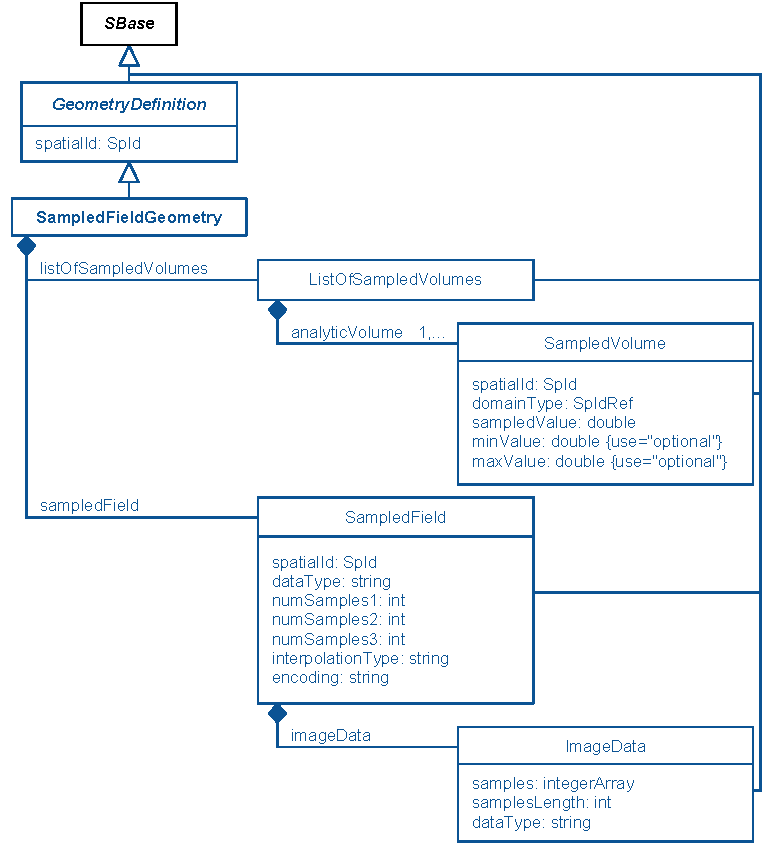
\includegraphics{figs/SampledFieldGeometry-uml}
  \caption{The definition of the \SampledFieldGeometry, \ListOfSampledVolumes, and \SampledVolume classes.}
  \label{SampledFieldGeometry-uml}
  \label{ListOfSampledVolumes-uml}
  \label{SampledVolume-uml}
\end{figure}

\subsubsection{The \fixttspace\tokenNC{sampledField} attribute}
The \token{sampledField} attribute is of type SpIdRef, and must reference a \SampledField from the same \Geometry.  That referenced field is to be used to set up the different spatial areas in the geometry of the \Model, according to the \SampledVolume child elements.

\subsection{The \class{SampledVolume} class}
\label{sampledvolume-class}
A \SampledVolume represents an interval of the sampled field that constitutes one or more contiguous regions. A \SampledVolume is defined for each volumetric (3-dimensional) \Domain in the \Geometry. Volumes are defined as regions within the referenced image that match a particular pixel value (\token{sampledValue}) or that match a range of pixel values (\token{minValue} and \token{maxValue}).  A given \SampledVolume must define for itself either a single value or a range of values to which it applies, but not both.  Within a \ListOfSampledVolumes, there must be at most one \SampledVolume that corresponds to any given pixel value.  That is, any given pixel value may only appear as the \token{sampledVolume} of a single \SampledVolume, or be between the \token{minValue} and \token{maxValue} (inclusive) of a single \SampledVolume.  It has the following attributes:

\subsubsection{The \fixttspace\tokenNC{id} and \fixttspace\tokenNC{name} attributes}
The \token{id} attribute identifies a \SampledVolume object. The attribute is of type \primtype{SpId} and is required when specifying a \SampledVolume.  It has no mathematical meaning, and cannot be connected to a \Parameter via a \SpatialSymbolReference element.  The optional \token{name} attribute is of type \primtype{string}, may be used to add a human-readable label to the object, and has no uniqueness requirements.

\subsubsection{The \fixttspace\tokenNC{domainType} attribute}
The required \token{domainType} attribute is of type \primtype{SpIdRef}. It is the \primtype{SpId} of the \DomainType that represents this class of anatomical features. If there are more than one contiguous regions, then more than one domain will be defined corresponding to each \SampledVolume.

\subsubsection{The \fixttspace\tokenNC{sampledValue} attribute}
The optional \token{sampledValue} attribute is of type \primtype{double}. It represents the pixel value of a \SampledVolume.  When used, all pixels with this particular value are to be assigned to this \SampledVolume, and no pixel without this value is assigned to the \SampledVolume.  It is illegal to define a \token{sampledValue} attribute for a \SampledVolume that also has a \token{minValue} and \token{maxValue} defined.

\subsubsection{The \fixttspace\tokenNC{minValue} attribute}
The optional \token{minValue} attribute is of type \primtype{double}. It represents the minimum of the pixel value (\token{sampledValue}) range to be assigned to this \SampledVolume.  If a \token{minValue} attribute is defined, a \token{maxValue} attribute must also be defined, and the \token{sampledValue} attribute must not be defined.  Areas in the \SampledField with \emph{exactly} this value are to be included in this \SampledVolume.

\subsubsection{The \fixttspace\tokenNC{maxValue} attribute}
The optional \token{maxValue} attribute is of type \primtype{double}. It represents the maximum of the pixel value (\token{sampledValue}) range to be assigned to this \SampledVolume.  If a \token{maxValue} attribute is defined, a \token{minValue} attribute must also be defined, and the \token{sampledValue} attribute must not be defined.  Areas in the \SampledField with \emph{exactly} this value are to be excluded from this \SampledVolume.

Having the \token{minValue} be included and the \token{maxValue} be excluded allows modelers to define adjacent volumes without ambiguity at the boundaries.  One \SampledVolume may be defined from 0 to 100, and a second volume defined from 100 to 200, and any location with a \SampledField value of exactly 100 is only assigned to the first \SampledVolume, and every location with a value close to 100 is included in exactly one \SampledVolume.


\subsection{\SampledFieldGeometry example}
\label{sampledfieldgeometry-example}
The following is an example of a sampled field geometry with three volumes.  The referenced \SampledField (defined in \sec{sampledfield-class}) is also included (though truncated).

\begin{example}
  <spatial:listOfGeometryDefinitions>
    <spatial:sampledFieldGeometry spatial:isActive="true" spatial:sampledField="imgvals">
      <spatial:listOfSampledVolumes>
        <spatial:sampledVolume spatial:id="Extracellular2" spatial:domainType="Extracellular"
                               spatial:minValue="0" spatial:maxValue="64"/>
        <spatial:sampledVolume spatial:id="Cytosol2" spatial:domainType="Cytosol2"
                               spatial:minValue="64" spatial:maxValue="192"/>
        <spatial:sampledVolume spatial:id="Nucleus2" spatial:domainType="Nucleus"
                               spatial:minValue="192" spatial:maxValue="256"/>
      </spatial:listOfSampledVolumes>
    </spatial:sampledFieldGeometry>
  </spatial:listOfGeometryDefinitions>
  <spatial:listOfSampledFields>
    <spatial:sampledField spatial:id="imgvals" spatial:dataType="uint8" spatial:numSamples1="51"
                          spatial:numSamples2="59" spatial:numSamples3="23"
                          spatial:interpolationType="linear" spatial:compression="uncompressed"
                          spatial:samplesLength="1255">
                                120 218 237 [...] 131 28 215
    </spatial:sampledField>
  </spatial:listOfSampledFields>
\end{example}

\subsection{The \class{CSGeometry} class}
\label{csgeometry-class}
\label{listofcsgobjects-class}
\CSGeometry (Constructed Solid Geometry) is a type of \GeometryDefinition that defines a combined, solid, volumetric object from a number of primitive solid volumes by the application of set operations such as union, intersection and difference and affine transformations such as rotation, scaling, translation, etc. The \CSGeometry element is defined by a \token{listOfCSGObjects} element that contains a collection of \CSGObjects. \fig{CSGeometry-uml} shows the definition of the \CSGeometry object.

\begin{figure}[ht]
  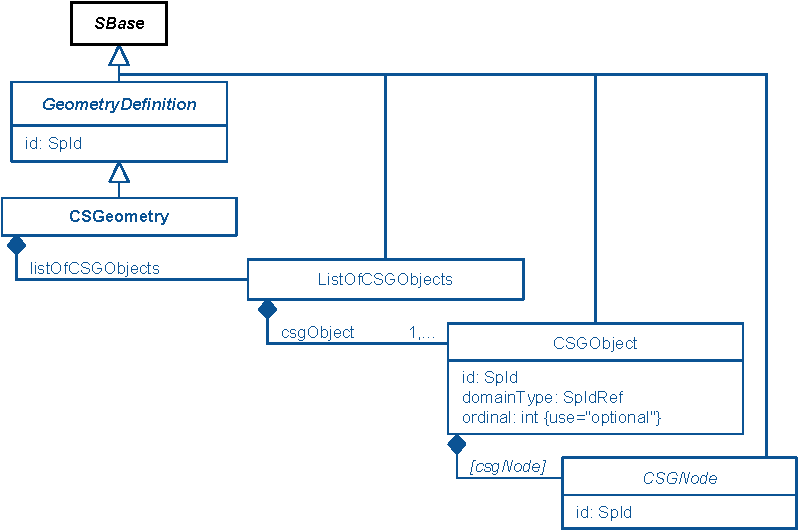
\includegraphics{figs/CSGeometry-uml}
  \caption{The definition of the \CSGeometry, \ListOfCSGObjects, and \CSGObject classes.}
  \label{CSGeometry-uml}
  \label{ListOfCSGObjects-uml}
  \label{CSGObject-uml}
\end{figure}



\subsection{The \class{CSGObject} class}
\label{csgobject-class}
Each \CSGObject is a scene graph representing a particular geometric object using constructed solid geometry. A node in a tree (scene graph) is made up of \CSGPrimitives, \CSGSetOperators, and \CSGTransformations.  Note that the \CSGPrimitives are always leaves in this tree. The \CSGObject is analogous to an \AnalyticVolume element in the sense that it is a constructed geometry (from primitives) used to specify a volumetric (3-dimensional) domain. The \CSGObject element has three attributes : \token{id}, \token{domainType} and \token{ordinal}. The definition of the \CSGObject is completed by defining a \CSGNode which is the root of the \CSGObject scene graph.

\subsubsection{The \fixttspace\tokenNC{id} and \fixttspace\tokenNC{name} attributes}
The \token{id} attribute uniquely identifies the \CSGObject element. The attribute is required and is of type \primtype{SpId}.  It has no mathematical meaning, and cannot be connected to a \Parameter via a \SpatialSymbolReference element.  The optional \token{name} attribute is of type \primtype{string}, may be used to add a human-readable label to the object, and has no uniqueness requirements.

\subsubsection{The \fixttspace\tokenNC{domainType} attribute}
The \token{domainType} attribute is of type \primtype{SpIdRef} and is a required attribute. It is a reference to the \token{id} of the \DomainType that this \CSGObject represents.

All \InteriorPoints of the corresponding \DomainType must be points inside the geometry this \CSGObject describes.


\subsubsection{The \fixttspace\tokenNC{ordinal} attribute}
The \token{ordinal} attribute is of type \primtype{int}.  It is used to represent the order of the \CSGObject. The \token{ordinal} is useful while reconstructing the geometry in the specific software tool - it represents the order in which the \CSGObjects representing geometric domains have to be placed.

No two \CSGObject elements should have the same \token{ordinal} value, even if they should not overlap, because some tools may not calculate the geometries to the same level of precision as other tools, and may end up with overlap due to rounding errors, and will still need to resolve the ambiguity for their own purposes.  If a software tool discovers two overlapping \CSGObject elements with the same \token{ordinal} value, it may resolve the situation however it sees fit.


\subsubsection{The [\tokenNC{csgNode}] child}

The child [\token{csgNode}] element represents the geometry that is to be linked to the \token{domainType} of the \CSGObject.  Note that the child of the \CSGObject element is not called \val{csgNode} but rather takes the name of the derived class, decapitalized.  Thus, a \CSGObject may have a \token{csgPrimitive}, \token{csgSetOperator}, \token{csgTranslation}, \token{csgRotation}, \token{csgScale}, or \token{csgHomogeneousTransformation} child.


\subsection{The \class{CSGNode} class}
\label{csgnode-class}
The operators and operands used to construct a constructed solid geometry are generalized as a \CSGNode, defined in \fig{CSGNode-uml} as an abstract base class. The classes that inherit from \CSGNode can be one of the following: \CSGSetOperator, \CSGTransformation (operators; itself another abstract base class), or \CSGPrimitive (operands). The \CSGNode has one attribute: \token{id}. The \CSGObject contains a \CSGNode object which is the root of the \CSGObject scene graph (representing one constructed solid geometry domain).

\begin{figure}[ht]
  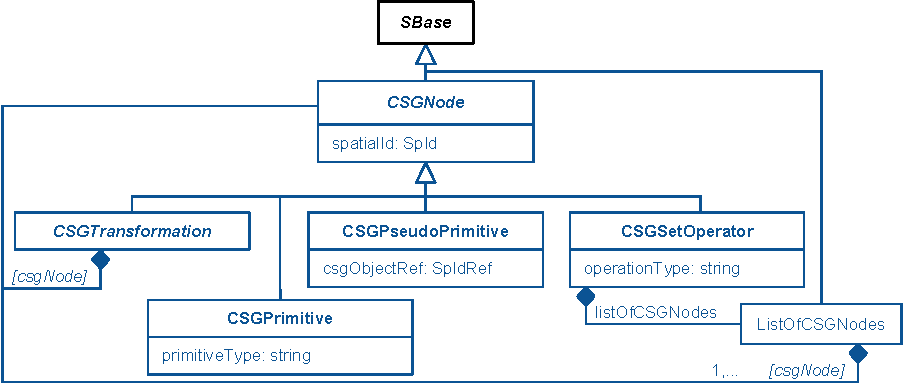
\includegraphics{figs/CSGNode-uml}
  \caption{The definition of the abstract base class \CSGNode, and its subclasses \CSGPrimitive, and \CSGSetOperator.  The abstract base class \CSGTransformation (also a subclass of \CSGNode) is defined in \sec{csgtransformation-class}.}
  \label{CSGNode-uml}
  \label{CSGPrimitive-uml}
%  \label{CSGPseudoPrimitive-uml}
  \label{CSGSetOperator-uml}
  \label{ListOfCSGNodes-uml}
\end{figure}

\subsubsection{The \fixttspace\tokenNC{id} and \fixttspace\tokenNC{name} attributes}
The \token{id} attribute uniquely identifies the \CSGNode element. The attribute is optional and is of type \primtype{SpId}.  It has no mathematical meaning, and cannot be connected to a \Parameter via a \SpatialSymbolReference element.  The optional \token{name} attribute is of type \primtype{string}, may be used to add a human-readable label to the object, and has no uniqueness requirements.


\subsection{The \class{CSGPrimitive} class}
\label{csgprimitive-class}
\CSGPrimitive element represents the primitive geometric shapes that can be represented by the \CSGeometry. These shapes are defined in \tab{primitive-definitions} with a predefined orientation and fitting within the unit cube (+/- 1 in x, y, and z) or unit square (+/- 1 in x and y). This element has one required attribute : \token{primitiveType} of type \primtype{PrimitiveKind}.

\subsubsection{The \fixttspace\tokenNC{primitiveType} attribute}
The \token{primitiveType} attribute is a required attribute that is of type \primtype{PrimitiveKind}. It represents one of the predefined primitive shapes.  The meaning and definition of those types is listed in \tab{primitive-definitions}.


\begin{table}[thb]
  \begin{edtable}{tabular}{>{\centering\arraybackslash}m{0.9in} >{\centering\arraybackslash}m{0.7in} >{\raggedright\arraybackslash}m{4.4in}}
  %\begin{edtable}{tabular}{p{0.9in}p{0.7in}p{4.4in}}
    \toprule
    \textbf{PrimitiveKind} & \textbf{Dimensions} & \textbf{Definition} \\
    \midrule
    \token{sphere}        & 3 & A sphere with radius 1, centered at the origin.\\
    \token{cube}          & 3 & A cube with sides of length 2, centered at the origin.\\
    \token{cylinder}      & 3 & A cylinder with a base circle of radius 1, centered at (0,0,-1), and top circle of radius 1, centered at (0,0,1).  The height is 2.\\
    \token{cone}          & 3 & A cone with a base circle of radius 1, centered at (0,0,-1), and top vertex at (0,0,1).\\
    \token{circle}        & 2 & A circle with radius 1, centered at the origin.\\
    \token{square}        & 2 & A square with sides of length 2, centered at the origin\\
    \bottomrule
  \end{edtable}
  \caption{Definitions of the possible values of the \token{primitiveType} attribute of the \CSGPrimitive class. 
} 
  \label{primitive-definitions}
\end{table}


%\subsection{The \class{CSGPseudoPrimitive} class}
%\label{csgpseudoprimitive-class}
%\CSGPseudoPrimitive element is used to reference a pre-defined \CSGObject object while defining a \CSGObject (geometric domain). This allows the re-use of one constructed \CSGObject in another. It has one attribute of type \primtype{SpIdRef}.

%\subsubsection{The \fixttspace\tokenNC{csgObjectRef} attribute}
%The \token{csgObjectRef} attribute identifies a pre-defined \CSGObject in the \CSGeometry The attribute is required and is of type \primtype{SpId}.  A \CSGObject may not reference itself, nor its parent, nor its parent's parent, etc.


\subsection{The \class{CSGSetOperator} class}
\label{csgsetoperator-class}
The \CSGSetOperator element represents the set operations (union, intersection, difference) that can be performed on a set of primitive geometric shapes (\CSGPrimitives) or on a set of \CSGNodes (a transformation or set operation on one or a set of \CSGPrimitives). This element has one attribute of type \primtype{string}. It also contains a required child \ListOfCSGNodes that represents the set of nodes on which the set operation is performed.

\subsubsection{The \fixttspace\tokenNC{operationType} attribute}
The \token{operationType} attribute is of type \primtype{SetOperation} and represents an operation that can be performed on a set of \CSGNodes. The possible values that the \token{operationType} attribute can take are \val{union}, \val{intersection}, or \val{difference}.  The values \val{union} and \val{intersection} are n-ary, meaning they are defined for any number of child nodes of this \CSGSetOperator.  The intersection or union of the empty set (zero children) is defined as the empty set, and the intersection or union of a single child is defined as that child.  The union of multiple sets is defined as including any element that appears in any of those component sets, and the intersection of multiple sets is defined as including only those elements that appear in all of the component sets.

The value \val{difference} is binary, meaning that it must have exactly two children.  Its meaning is defined according to the \token{complement} attributes, below.

\subsubsection{The \fixttspace\tokenNC{complementA} and \tokenNC{complementB} attributes}
The \token{complement} attributes are of type \primtype{SpIdRef}.  If the \token{operationType} of the \CSGSetOperator has the value \val{difference}, they both must be set to indicate the order in which the complement is to be carried out, and must refer, respectively, to the two \token{csgNode} children of this \CSGSetOperator.  The relative complement of the children (and thus the meaning of this node) is defined as the set of elements in \token{complementB}, but not in \token{complementA}.  

If the \token{operationType} of the \CSGSetOperator is not \val{difference}, neither \token{complement} attribute may be set.



\subsection{The \class{ListOfCSGNodes} class}
\label{listofcsgnodes-class}
The \ListOfCSGNodes must contain one or more \token{csgNode} children that are to be combined according to the set operation of the parent \CSGSetOperator.  While having a single child is legal, this is semantically equivalent to simply putting that child in the model instead of the \CSGSetOperator, and therefore has limited modeling benefit.  Note that the children of the \ListOfCSGNodes object are not called \token{csgNode} but rather take the name of the derived class, decapitalized.  Thus, they may be called \token{csgPrimitive}, \token{csgSetOperator}, \token{csgTranslation}, \token{csgRotation}, \token{csgScale}, or \token{csgHomogeneousTransformation}.


\subsection{The \class{CSGTransformation} class}
\label{csgtransformation-class}
The \CSGTransformation represents a generalization for the type of transformation that can be performed on a primitive geometric shape (\CSGPrimitive) or on a \CSGNode (a transformation or set operation on one or a set of \CSGPrimitives). The types of possible transformations are 'rotation', 'translation', 'scaling', and 'homogeneous transformation', defined below. The \CSGTransformation element contains a \CSGNode element upon which the transformation is performed.

Each transformation is performed directly on its child \CSGNode, with any transformation or set operation from that node already performed.  This essentially defines a 'bottom-up' approach, where the tips of the XML tree children of a \CSGObject are all \CSGPrimitive objects, that are progressively transformed or combined with other \CSGPrimitive objects by each successive node moving rootward through the XML.  For an example, see \sec{csgobject-example}.

\begin{figure}[ht]
  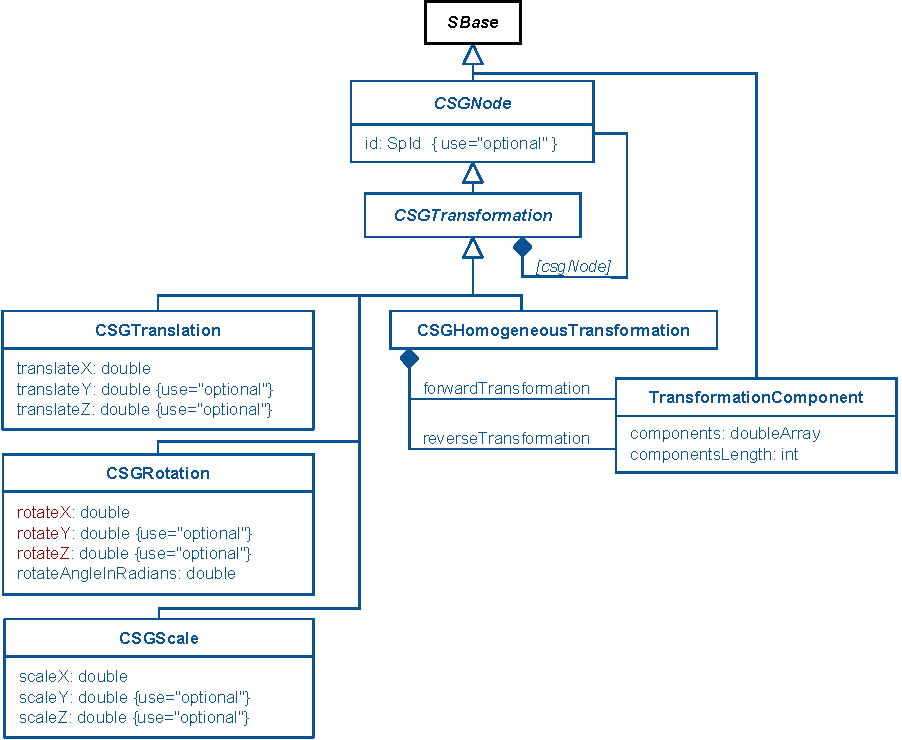
\includegraphics{figs/CSGTransformation-uml}
  \caption{The definition of the abstract base class \CSGTransformation, its subclasses (\CSGTranslation, \CSGRotation, \CSGScale, and \CSGHomogeneousTransformation), and the \TransformationComponent class.}
  \label{CSGTransformation-uml}
  \label{CSGRotation-uml}
  \label{CSGScale-uml}
  \label{CSGHomogeneousTransformation-uml}
  \label{TransformationComponent-uml}
\end{figure}

\subsubsection{The \fixttspace\tokenNC{csgNode} child}

The child \token{csgNode} element represents the geometry that is to be transformed by the \CSGTransformation element.  Note that this child is not called \token{csgNode} but rather takes the name of the derived class, decapitalized.  Thus, it may be called \token{csgPrimitive}, \token{csgSetOperator}, \token{csgTranslation}, \token{csgRotation}, \token{csgScale}, or \token{csgHomogeneousTransformation}.


\subsection{The \class{CSGTranslation} class}
\label{csgtranslation-class}
The \CSGTranslation element represents a translation transformation on a \CSGNode (a transformation or set operation on one or a set of \CSGPrimitives) or a \CSGPrimitive along the axes defined in the \Geometry. This element has 3 attributes:

\subsubsection{The \fixttspace\tokenNC{translateX} attribute}
The \token{translateX} required attribute is of type \primtype{double}. It represents the translation of the \CSGNode along the x-axis (the \CoordinateComponent with the \token{type} of \val{cartesianX}).

\subsubsection{The \fixttspace\tokenNC{translateY} attribute}
The \token{translateY} attribute is of type \primtype{double}. It represents the translation of the \CSGNode along the y-axis (the \CoordinateComponent with the \token{type} of \val{cartesianY}).  This attribute must not be defined if no such \CoordinateComponent is present in the parent \Geometry, and is required otherwise.

\subsubsection{The \fixttspace\tokenNC{translateZ} attribute}
The \token{translateZ} attribute is of type \primtype{double}. It represents the translation of the \CSGNode along the z-axis (the \CoordinateComponent with the \token{type} of \val{cartesianZ}).  This attribute must not be defined if no such \CoordinateComponent is present in the parent \Geometry, and is required otherwise.

%Note:  we'll have to change the above if we ever re-introduce non-cartesian coordinates.

\subsection{The \class{CSGRotation} class}
\label{csgrotation-class}
The \CSGRotation element represents a rotation transformation on a \CSGNode (a transformation or set operation on one or a set of \CSGPrimitives) or a \CSGPrimitive about the axes defined in the \Geometry. This element has 4 attributes:

\subsubsection{The \fixttspace\tokenNC{rotateX}, \tokenNC{rotateY}, and \tokenNC{rotateZ} attributes}
The \token{rotate} attributes are of type \primtype{double}, and must be defined for the same number of \CoordinateComponents as are present in the parent \Geometry.  If all three are defined, they define a point in space that determines the vector (from the origin) of the axis about which the rotation is to occur in three-dimensional space.  They must therefore not all be equal to zero.  If two are defined (\token{rotateX} and \token{rotateY}), they define the point in two-dimensional space about which the rotation is to occur.  (In this case, (0,0) would be legal.)  Nothing can be rotated in 1-dimensional space, and therefore defining only \token{rotateX} is meaningless.

\subsubsection{The \fixttspace\tokenNC{rotateAngleInRadians} attribute}
The \token{rotateAngleInRadians} attribute is of type \primtype{double}. It represents the rotation angle of the \CSGNode, in radians, along the defined axis.  In three-dimensional space, this rotation is defined as counterclockwise from the perspective of the origin, viewing the constructed vector.  In two-dimensional space, this rotation is defined the same way, as a counterclockwise rotation along the Z axis emerging from the defined point.  From the perspective of the surface of the shape, this view looks down the negative side of the Z axis, appearing as a clockwise rotation.

Overall, the \token{rotate} attributes define \emph{where} the rotation is to occur, and the \token{rotateAngleInRadians} define \emph{how much} rotation is to take place.  A \token{rotateAngleInRadians} value of \val{0} would therefore define a \CSGRotation that left the shape fixed in space.


\subsection{The \class{CSGScale} class}
\label{csgscale-class}
The \CSGScale element represents a scale transformation on a \CSGNode (a transformation or set operation on one or a set of \CSGPrimitives) or a \CSGPrimitive along the axes defined in the \Geometry.  All scaling occurs collectively for the component primitive shapes, and the expansion occurs from the geometrical center of the object, i.e. the center of the smallest bounding box that would contain the current volume of the object.  This means, for example, that if the child of the \CSGScale object is a hemisphere, defined as the intersection of a sphere and a cube, the bounding box would be half the size of a box that would have included the original entire sphere.

This element has 3 attributes:

\subsubsection{The \fixttspace\tokenNC{scaleX} attribute}
The \token{scaleX} required attribute is of type \primtype{double}. It represents the amount of scaling of the \CSGNode along the x-axis (the \CoordinateComponent with the \token{type} of \val{cartesianX}).

\subsubsection{The \fixttspace\tokenNC{scaleY} attribute}
The \token{scaleY} attribute is of type \primtype{double}. It represents the amount of scaling of the \CSGNode along the y-axis (the \CoordinateComponent with the \token{type} of \val{cartesianY}).  This attribute must not be defined if no such \CoordinateComponent is present in the parent \Geometry, and is required otherwise.

\subsubsection{The \fixttspace\tokenNC{scaleZ} attribute}
The \token{scaleZ} attribute is of type \primtype{double}. It represents the amount of scaling of the \CSGNode along the z-axis (the \CoordinateComponent with the \token{type} of \val{cartesianZ}).  This attribute must not be defined if no such \CoordinateComponent is present in the parent \Geometry, and is required otherwise.

The amount of scaling for all three attributes is relative to the original size of the object.  In other words, if a \CSGScale object has a \token{scaleX} value of \val{1.0}, is it not scaled along the X axis at all, with \val{0.5} halving it, \val{2.0} doubling it, and \val{0.0} making the entire object disappear completely.  Negative values produce effective inversions of the object, e.g. inverting a unit cone by giving it a \token{scaleZ} scaling factor of \val{-1}.


\subsection{The \class{CSGHomogeneousTransformation} class}
\label{csghomogeneoustransformation-class}
The \CSGHomogeneousTransformation element represents a homogeneous transformation on a \CSGNode: a transformation or set operation on one or more \CSGPrimitives. This element contains one required \TransformationComponent element child named \token{forwardTransformation}.

%{\color{red} Lucian: \notice Still trying to track down whether anyone has implemented 'reverseTransformation'.  If not, we'll remove it from the spec as unnecessary, and just leave 'forwardTransformation'.}


\subsection{The \class{TransformationComponent} class}
\label{transformationcomponent-class}
The \TransformationComponent element represents an affine transformation that can be applied to a \CSGNode. This element has the following two attributes:

\subsubsection{The \fixttspace\tokenNC{components} attribute}
The \token{components} attribute is of type \primtype{doubleArray}, whose values represent the 4x4 affine transformation matrix. This attribute is required.

An affine transformation is essentially a method to transform a shape's scale, rotation, and translation all at once instead of breaking it down into its component tranformations.  For one description of how to transform a model with an affine transformation, see the OpenGL Programming Guide, Chapter 5 \citep{shreiner2013opengl}.

%{\color{red} Lucian: \notice If someone can concisely explain the algorithm at work here, and can send it to me, I will put it into the spec, because despite reading up on affine transformations on Wikipedia, I don't understand it well enough to explain how you get from a vector of components to a transformed shape.}


\subsubsection{The \fixttspace\tokenNC{componentsLength} attribute}
The \token{componentsLength} attribute is of type \primtype{int}, is required, and must be 16. It represents the array length of the \token{components} attribute (number of values in the \token{components} array), which must be a 4x4 matrix.


\subsection{CSGObject examples}
\label{csgobject-example}
The following is an example of a \CSGObject which has been scaled, rotated, and translated:

\begin{example}
  <spatial:csgObject spatial:id="vesicleObj" spatial:domainType="vesicle"
                     spatial:ordinal="2">
    <spatial:csgTranslation spatial:id="translation1" spatial:translateX="5.439"
                            spatial:translateY="5.88" spatial:translateZ="1.078">
      <spatial:csgRotation  spatial:id="rotation1" spatial:rotateX="2.4391"
                            spatial:rotateY="1.5373" spatial:rotateZ="0.58404"
                            spatial:rotateAngleInRadians="0.9104">
        <spatial:csgScale   spatial:id="scale1" spatial:scaleX="0.075833"
                            spatial:scaleY="0.080451" spatial:scaleZ="0.029583">
          <spatial:csgPrimitive spatial:id="sphere1" spatial:primitiveType="sphere"/>
       </spatial:csgScale>
      </spatial:csgRotation>
    </spatial:csgTranslation>
  </spatial:csgObject>
\end{example}

The manipulations can be read from the inside out: at the base level, we have the \CSGPrimitive sphere: a sphere with radius 1.0, centered at the origin.  It's then scaled such that it is compressed along each axis by different amounts: along the X axis to 7.5833\%, along the Y axis to 8.0451\%, and along the Z axis to 2.9583\%.  Then the scaled figure is rotated around a vector with its origin at (0,0,0) and its point at (2.4391, 1.5373, 0.58404), by 0.9104 radians.  Finally, it is translated by 5.439 along the X axis, 5.88 along the Y axis, and 1.078 along the Z axis.

In this second example, a hemisphere is created through the intersection of a primitive sphere and translated cube:

\begin{example}
  <spatial:csgObject spatial:id="hemisphere" spatial:domainType="Nucleus">
    <spatial:csgSetOperator spatial:operationType="intersection">
      <spatial:listOfCSGNodes>
        <spatial:csgPrimitive spatial:primitiveType="sphere"/>
        <spatial:csgTranslation spatial:translateX="1" spatial:translateY="0"
                                spatial:translateZ="0">
          <spatial:csgPrimitive spatial:primitiveType="cube"/>
        </spatial:csgTranslation>
      </spatial:listOfCSGNodes>
    </spatial:csgSetOperator>
  </spatial:csgObject>
\end{example}


\subsection{The \class{ParametricGeometry} class}
\label{parametricgeometry-class}
\label{listofparametricobjects-class}
\ParametricGeometry is a type of \GeometryDefinition that parametrically defines geometric strucutures/domains. The \ParametricGeometry element is defined with a \SpatialPoints object and a \token{listOfParametricObjects} that is a collection of \ParametricObjects. Each point in the \SpatialPoints list is given an index, and those indices are used in the creation of each \ParametricObject.  There may be points whose indices are never used; this does not affect the \ParametricGeometry.  \fig{ParametricGeometry-uml} shows the definition of the \ParametricGeometry object.

\begin{figure}[ht]
  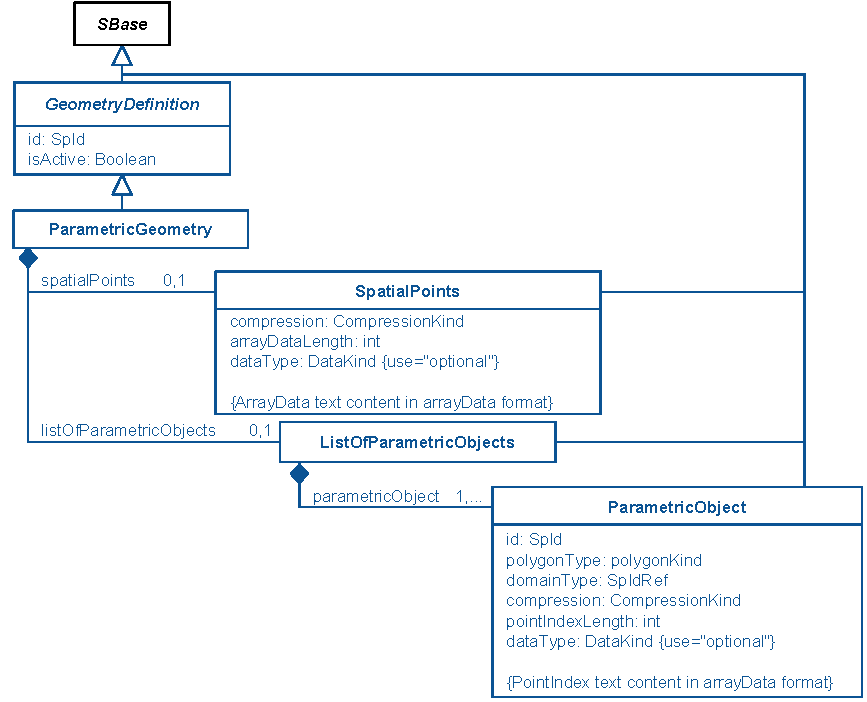
\includegraphics{figs/ParametricGeometry-uml}
  \caption{The definition of the \ParametricGeometry, \SpatialPoints, \ListOfParametricObjects, and \ParametricObject classes.}
  \label{ParametricGeometry-uml}
  \label{SpatialPoints-uml}
  \label{ListOfParametricObjects-uml}
  \label{ParametricObject-uml}
  \label{PolygonObject-uml}
\end{figure}


\subsection{The \class{SpatialPoints} class}
\label{spatialpoints-class}
The \SpatialPoints element represents the set of points to be used as vertices in the \ParametricGeometry.  In essence, the \SpatialPoints defines a lattice on which each \ParametricObject is to be drawn.  There may be unused points in the list if no \ParametricObject ever uses that index to draw its shape.

\subsubsection{The \fixttspace\tokenNC{compression} attribute}
The required \token{compression} attribute is of type \primtype{CompressionKind}. It is used to specify the compression used when encoding the data, and can have the value \val{uncompressed} if no compression was used, or \val{deflated} if the deflation algorithm was used to compress the data. \changed{The deflation compression algorithm to be used is gzip, which adds a header to the deflated data.  This algorithm is freely available.  The version of the data to be compressed is the string version of the values in the array, which may consist of numbers, whitespace, commas, and semicolons.}

%{\color{red} Lucian: \notice Based on our discussion on the list about compression, the above is a compromise/temporary position so that existing implementations can continue to work for now, but we are moving towards using base64 in the future. Eventually, if base64 turns out to work great, we should be able to drop 'deflated' as an option entirely, and only use 'uncompressed' and 'base64'.}

\subsubsection{The \fixttspace\tokenNC{arrayDataLength} attribute}
The \token{arrayDataLength} attribute is of type \primtype{int} and is required. It represents the array length of the \primtype{arrayData} text child of this node.  If uncompressed, this will equal the total number of coordinates, but if compressed, this will equal the new compressed length of the array, not including any added whitespace.  It is included for convenience and validation purposes.


\subsubsection{The \fixttspace\tokenNC{dataType} attribute}
The \token{dataType} attribute is of type \primtype{DataKind} and is optional.  It is used to specify the type of the data being stored\changed{, so that the uncompressed data can be stored in an appropriate storage type.  The three main value types are \val{uint} for unsigned integers, \val{int} for signed integers, and \val{double} for double-precision floating point values.  For backwards compatibility, and for cases where storage space might be an issue, other values may also be used:} \val{float} to indicate single-precision (32-bit) floating point values, and \val{uint8}, \val{uint16}, and \val{uint32} to indicate 8-bit, 16-bit, and 32-bit unsigned integer values, respectively.

\subsubsection{The \fixttspace\tokenNC{ArrayData} text child}
The \token{ArrayData} text child of the \SpatialPoints is in \token{arrayData} format, and represents an ordered list of sets of coordinates that will be used as the vertices of \ParametricObject elements in this \ParametricGeometry, with \val{0} representing the first such coordinate, \val{1} the second, etc.  The list will define vertexes with as many values as there are \CoordinateComponent children of the parent \Geometry:  three values for representing the X, Y, and Z coordinates (respectively) of 3-dimensional geometries, or two values for representing the X and Y coordinates (respectively) of 2-dimensional geometries.  (\ParametricGeometry elements cannot be created in 1-dimensional geometries.)  It is suggested, but not required, that if the data is uncompressed, that the grouped points be separated from each other with the use of a semicolon.  If the data is compressed, a semicolon is not to be used.

\begin{blockChanged}
\subsubsection{The \fixttspace\tokenNC{id} and \fixttspace\tokenNC{name} attributes}
Each \SpatialPoints is identified with a \token{id} of type \primtype{SpId}.  A \SpatialPoints has no mathematical value.  The optional \token{name} attribute is of type \primtype{string}, may be used to add a human-readable label to the object, and has no uniqueness requirements.
\end{blockChanged}


\subsection{The \class{ParametricObject} class}
\label{parametricobject-class}
The \ParametricObject element represents a single parametric geometry object.  It contains a list of point indices from the parent \ParametricGeometry's \SpatialPoints, which collectively define the faces of the object.

\subsubsection{The \fixttspace\tokenNC{id} and \fixttspace\tokenNC{name} attributes}
The \token{id} attribute is a required attribute of type \primtype{SpId}. It uniquely identifies the \ParametricObject element.  It has no mathematical meaning, and cannot be connected to a \Parameter via a \SpatialSymbolReference element.  The optional \token{name} attribute is of type \primtype{string}, may be used to add a human-readable label to the object, and has no uniqueness requirements.

\subsubsection{The \fixttspace\tokenNC{polygonType} attribute}
The \token{polygonType} attribute is of type \primtype{PolygonKind} and is a required attribute. It represents the type of polygon that describes the \ParametricObject.  \ParametricObject elements of type \val{triangle} have three points, and those of type \val{quadrilateral} have four.

\subsubsection{The \fixttspace\tokenNC{domainType} attribute}
The \token{domainType} attribute is of type \primtype{SpIdRef} and is a required attribute. It is a reference to the \token{id} of the \DomainType that this \ParametricObject represents.

\subsubsection{The \fixttspace\tokenNC{compression} attribute}
The required \token{compression} attribute is of type \primtype{CompressionKind}. It is used to specify the compression used when encoding the data, and can have the value \val{uncompressed} if no compression was used, or \val{deflated} if the deflation algorithm was used to compress the data.  \changed{The deflation compression algorithm to be used is gzip, which adds a header to the deflated data.  This algorithm is freely available.  The version of the data to be compressed is the string version of the values in the array, which may consist of numbers, whitespace, commas, and semicolons.}

%{\color{red} Lucian: \notice Based on our discussion on the list about compression, the above is a compromise/temporary position so that existing implementations can continue to work for now, but we are moving towards using base64 in the future. Eventually, if base64 turns out to work great, we should be able to drop 'deflated' as an option entirely, and only use 'uncompressed' and 'base64'.}

\subsubsection{The \fixttspace\tokenNC{pointIndexLength} attribute}
The \token{pointIndexLength} attribute is of type \primtype{int} and is required. It represents the array length of the \primtype{arrayData} text child of this node.  If uncompressed, this will equal the number of referenced indices, but if compressed, this will equal the new compressed length of the array, not including any added whitespace.  It is included for convenience and validation purposes.

\subsubsection{The \fixttspace\tokenNC{dataType} attribute}
The \token{dataType} attribute is of type \primtype{DataKind} and is optional.  It is used to specify the type of the data being stored\changed{, so that the uncompressed data can be stored in an appropriate storage type.  Because all the data will be indexes into the \token{ArrayData} of the \SpatialPoints element, \val{uint} is the suggested value for this attribute (indicating unsigned integer values), with \val{uint8}, \val{uint16}, and \val{uint32} (indicating 8-bit, 16-bit, and 32-bit unsigned integer values, respectively) also being allowed.  No other value is allowed, including the other types of \primtype{DataKind} (\val{int}, \val{float}, and \val{double}), since the data will never be that type.}


\subsubsection{The \fixttspace\tokenNC{PointIndex} text child}
The \token{PointIndex} text child of the \ParametricObject is in \token{arrayData} format, and represents an ordered list of indices that refer to elements in the \SpatialPoints array and are interpreted by considering the \token{polygonType} attribute of the \ParametricObject with a value of \val{triangle} indicating that the data is to be grouped in sets of three, and a value of \val{quadrilateral} indicating that the data is to be grouped in sets of four.  The sequence of indices must follow adjacent edges, with an implied edge between the first and last vertex.  Additionally, the order of that sequence should be consistently clockwise or counter-clockwise for any contiguous surface.  This can be accomplished by ensuring that when an edge is used for two different faces, the order of that edge is reversed for the second face.  It is suggested, but not required, that if the data is uncompressed, that the grouped points be separated from each other with the use of a semicolon.  If the data is compressed, a semicolon is not to be used.  Each set of indices that define a polygon face should each refer to a different location.  This means that one should not re-use index values with a single polygon face, nor should one use two index values in the same face that are mapped to the same location.

\subsection{A \class{ParametricGeometry} example}
\label{parametricgeometry-example}

As an example, if the \SpatialPoints element in a three-dimensional \Geometry is:

\begin{example}
    <spatialPoints compression="uncompressed" arrayDataLength="24">
        0 0 0; 0 0 1; 0 1 0; 1 0 0; 0 1 1; 1 0 1; 1 1 0; 1 1 1
    </spatialPoints>
\end{example}

This defines eight points, with point '0' at coordinates [0, 0, 0], point '1' at coordinates [0, 0, 1], etc., that happen to form the vertexes of a cube.  These point indexes are then used in the following \ParametricObject:

\begin{example}
    <parametricObject id="pyramid" polygonType="triangle" domainType="dt1"
                      compression="uncompressed" pointIndexLength="12">
        0 2 5; 0 6 2; 0 5 6; 2 6 5
    </parametricObject>
\end{example}

This defines a pyramid with four triangular faces.  The first triangle is defined by points [0,0,0], [0,1,0], and [0,1,1]; the second triangle by points [0,0,0], [1,1,0], and [0,1,0]; the third by [0,0,0], [0,1,1], and [1,1,0]; and the fourth by [0,1,0], [1,1,0], and [0,1,1].  Note also that the order of the faces is consistent, defining each face in a counter-clockwise order, as observed from 'outside' the pyramid.  This can be seen, for example, in the last two faces defined, where the shared edge is defined in the order '5 6' in the first face, but '6 5' in the second.

A more realistic example can be found below, though most of the values are elided for reasons of space:

\begin{example}
  <spatial:parametricGeometry spatial:id="id051101043048054" spatial:isActive="true">
    <spatial:spatialPoints spatial:compression="uncompressed" spatial:arrayDataLength="179901">
          -0.472894296 -0.4420042305 -0.457890447 [...]
          0.830988196507629 0.857225748552666 0.827138489800772
    </spatial:spatialPoints>
    <spatial:listOfParametricObjects>
      <spatial:parametricObject spatial:id="nucObj" spatial:polygonType="triangle"
                                spatial:domainType="nuc" spatial:pointIndexLength="24414"
                                spatial:compression="uncompressed">
          69 225 253 247 217 24 181 451 452 [...] 732 2417 3925
      </spatial:parametricObject>
      <spatial:parametricObject spatial:id="cellObj" spatial:polygonType="triangle"
                                spatial:domainType="cell" spatial:pointIndexLength="46242"
                                spatial:compression="uncompressed">
          423 8 418 2240 439 180 187 97 299 [...] 8197 1262 3043
      </spatial:parametricObject>
    </spatial:listOfParametricObjects>
  </spatial:parametricGeometry>
\end{example}

Here, an array of 179901 values is defined in the \SpatialPoints object.  Because this is a model with 3D geometry (described elsewhere in the model), the points are grouped in threes, with the first value representing the X value for the first point, the second value the Y of the first point, and the third the Z value of the first point.  The next value (elided) would be the X value of the second point, etc., until the final three values encode the final point, for a total of 59967 points (179901/3).  The first point (-0.472894296, -0.4420042305, -0.457890447) is referenced by its index of \val{0}, the second by its index of \val{1}, etc., through (0.830988196507629, 0.857225748552666, 0.827138489800772) for the point with index 59966.

These points are then used as in two meshes: one for the nucObj, and one for the cellObj.  Because both have the \token{polygonType} \val{triangle}, the list of points are intrepreted in groups of three:  (69, 225, 253) being the three vertices of the first triangle of \val{nucObj}, (245, 217, 24) the vertices of the second, etc.  Similarly, (423, 8, 418) is the first defined triangle for \val{cellObj}, and (8197, 1262, 3043) the last.

Because so many values were included, a decision was made to omit the optional \val{;} characters, which would have principally served to increase the file size.


\subsection{The \class{MixedGeometry} class}
\label{mixedgeometry-class}
\label{listofordinalmappings-class}

A \MixedGeometry defines a \Geometry constructed from a collection of various \GeometryDefinition objects that together define the complete geometry for the \Model.  It has a child \ListOfGeometryDefinitions object that behaves exactly the same as the \ListOfGeometryDefinitions child of the \Geometry, but instead of that collection of geometry definitions defining alternate geometries, or alternate ways to define one geometry, the collection of geometry definitions in a \MixedGeometry together define a single space.  For example, a \MixedGeometry may contain a \ParametricGeometry that defines the contours of a cell membrane, plus a \CSGeometry that defines a sphere that models the nucleus of that cell.  The definition of a \MixedGeometry is shown in \fig{mixedgeometry-uml}.  Its \OrdinalMapping children define how those geometries overlap one another.

Note that every child \GeometryDefinition of a \MixedGeometry must have an \token{isActive} value of \val{false}.  'Active' geometries are a concept that applies only to the \Model and its direct children, not to component geometries of a \MixedGeometry.  

\begin{figure}[ht]
  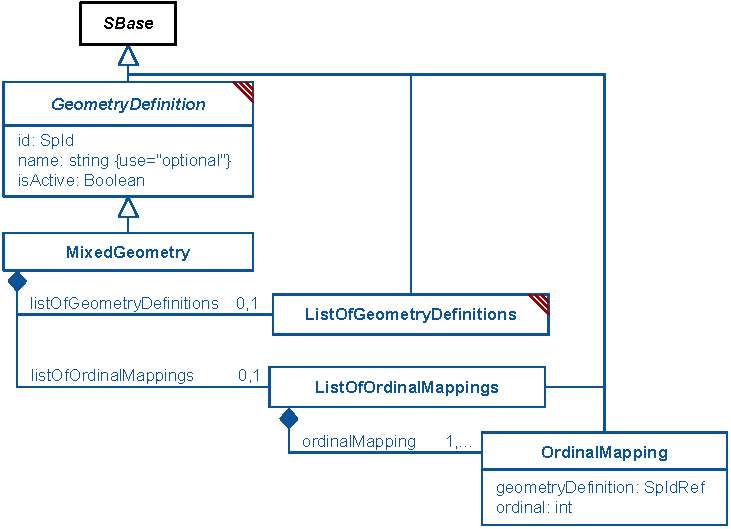
\includegraphics{figs/MixedGeometry-uml}
  \caption{The definition of the \MixedGeometry, \ListOfOrdinalMappings, and \OrdinalMapping classes from the Spatial package.  The \ListOfGeometryDefinitions class is defined in \sec{listofgeometrydefinitions-class}}
  \label{mixedgeometry-uml}
\end{figure}

\subsection{The \class{OrdinalMapping} class}
\label{ordinalmapping-class}
A \OrdinalMapping defines an ordinal level for the various geometries that comprised this \MixedGeometry.  In this way, the overlap between them can be resolved cleanly.  There must be exactly one \OrdinalMapping for each child \GeometryDefinition of a \MixedGeometry.

%{\color{red} Lucian: \notice Or we could make that a 'should'?  'ordinal' is required in the other places it is used, so 'must' is parallel to that.}


\subsubsection{The \fixttspace\tokenNC{geometryDefinition} attribute}
The token{geometryDefinition} attribute is of type \primtype{SpIdRef}, and is required.  It must reference a direct child \GeometryDefinition of this \MixedGeometry.  The \token{ordinal} value is then taken to refer to that geometry.


\subsubsection{The \fixttspace\tokenNC{ordinal} attribute}
The \token{ordinal} attribute is of type \primtype{int}, and is required. It is used to represent the order of the corresponding \GeometryDefinition within this \MixedGeometry.  The \token{ordinal} is useful while reconstructing the geometry in the specific software tool - it represents the order in which each \GeometryDefinition have to be evaluated.

Rather than struggle with the task of preventing overlapping regions of space from each different \GeometryDefinition, they are to be considered to be evaluated in the reverse order of their ordinals.  In this way, any \GeometryDefinition that has already been processed will cover those with a smaller ordinal, thus resolving any ambiguities and removing the constraint that each \GeometryDefinition be disjoint and cover the entire geometric domain.  The \GeometryDefinition with \token{ordinal} 0 can be the "background" layer (typically the extracellular space).  

No two \GeometryDefinition elements should have the same \token{ordinal} value, even if they should not overlap, because some tools may not calculate the geometries to the same level of precision as other tools, and may end up with overlap due to rounding errors, and will still need to resolve the ambiguity for their own purposes.  If a software tool discovers two overlapping \GeometryDefinition elements with the same \token{ordinal} value, it may resolve the situation however it sees fit.

Note that these ordinals only apply at the level of the immediate parent \MixedGeometry.  Any \token{ordinal} attribute from any \AnalyticVolume or \CSGObject applies only at the level of those volumes or objects, and serve to distinguish within-\GeometryDefinition layout order, not between-\GeometryDefinition layout order, defined here.  Likewise, if a \GeometryDefinition child of a \MixedGeometry it itself a \MixedGeometry, those ordinals also only apply at the level of that \MixedGeometry, and not at the level of the parent \MixedGeometry.


\subsection{The \class{SampledField} class}
\label{sampledfield-class}
A \SampledField is a sampled scalar field such as an image or samples from a level set. The attributes of \SampledField represent the specification of a sample dataset (the number of samples in x, y, z coordinates, data type of the sample representation, etc.) and the text child of the \SampledField is the actual sampled data, defined in \fig{sampledfield-uml}.  The purpose of a \SampledField is to fill the \Geometry with values that can be used in math and/or in \SampledFieldGeometry elements.  Values are defined at lattice points within the \Geometry, and are interpolated to fill the remainder of all off-lattice locations.

\begin{figure}[ht]
  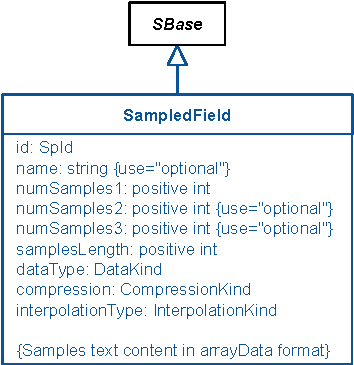
\includegraphics{figs/SampledField-uml}
  \caption{The definition of the \SampledField class from the Spatial package.}
  \label{sampledfield-uml}
\end{figure}

\subsubsection{The \fixttspace\tokenNC{id} and \fixttspace\tokenNC{name} attributes}
The \token{id} attribute identifies a \SampledField.  It is of type \primtype{SpId} and is a required attribute.  The mathematical value of a \SampledField is the value and dimensionality of the field itself, and can be bound to a \Parameter by using a \SpatialSymbolReference.  If used in conjunction with the SBML Level~3 \val{arrays} package, it can be used and manipulated as if it was an array of the appropriate dimensions, even though its \emph{meaning} is the value of the field at all points within its borders, not just those at the lattice points.  However, even without the use of the \val{arrays} package, it can be used in \sbmlthreecore MathML to set the value of a spatially-distributed SBML symbol such as a \Species or \Parameter, such as through an \InitialAssignment, \Rule, or \EventAssignment.  The optional \token{name} attribute is of type \primtype{string}, may be used to add a human-readable label to the object, and has no uniqueness requirements.

The size of the field is assumed to match the axes (the \CoordinateComponent children) of the parent \Geometry, and is assumed to be regularly spaced in each dimension, but is not required to be spaced the same way in all dimensions.  In other words, if the Geometry defines a 10 cm by 10 cm square, and a SampledField is a 10x5 array, the \val{[0,0]} entry in the array will correspond to the point \val{0~cm, 0~cm} in the Geometry, and the \val{[10,5]} entry in the array will correspond to the point \val{10~cm, 10~cm} in the Geometry.  Off-latice points (such as the value at \val{9~cm, 9~cm} in this example) have no direct corresponding value in the \SampledField, and are determined according to the \token{interpolationType} attribute, defined below.

When tied to a \SpatialSymbolReference, regardless of its useage, each \SampledField still must represent values across the entire \Geometry.  If used in an \InitialAssignment to assign values to a \Species that only exists in a particular \DomainType within the \Geometry, entries in the \SampledField that correspond to areas of space not covered by that \DomainType will simply be ignored.  Those values may be set to zero, or could be used in other contexts.  For example, a \SampledField could represent 'the concentration of ATP in the Geometry', and one \InitialAssignment could be used to apply the field to the species 'ATP in the cytosol' and a second \InitialAssignment could be used to apply the same field to the species 'ATP in the nucleus', with different values being examined and used in each case.

When used in a \SampledFieldGeometry, again, the values of the field are interpolated to all off-lattice points to determine whether or not any arbitrary location within the \Geometry is part of a given \SampledVolume or not.

%{\color{red} Lucian: \notice Is the above description reasonable?}

\subsubsection{The \fixttspace\tokenNC{interpolationType} attribute}
The required \token{interpolationType} attribute is type \primtype{InterpolationKind}. It is used to specify how values at off-lattice locations are to be calculated.  A value of \val{nearestNeighbor} means that the nearest lattice point value is to be returned.  A value of \val{linear} means that the value to be returned is the linear interpolation from nearby lattice points, either simple linear in the case of one-dimensional interpolation, bilinear in the case of two-dimensional interpolation, or trilinear in the case of three-dimensional interpolation.

%If the attribute is not defined, then no interpolation strategy is to be inferred or implied for this \SampleData element.  Simulators may use one of the above strategies or some other strategy, as befits their situation.

\subsubsection{The \fixttspace\tokenNC{numSamples1}, \tokenNC{numSamples2}, \tokenNC{numSamples3} attributes}
The \token{numSamples1}, \token{numSamples2}, and \token{numSamples3} attributes represent the number of samples in each of the coordinate components. (e.g. numX, numY, numZ) in an image dataset.  These attributes are of type \primtype{positive int} and are required to specify the \SampledField. The samples are assumed to be uniformly sampled.  It is required to have as many \token{numSamples} attributes as there are \CoordinateComponent elements in the \Geometry, with \token{numSamples1} defined if there is a \token{cartesianX} element; \token{numSamples2} defined if there is a \token{cartesianY} element, and \token{numSamples3} defined if there is a \token{cartesianZ} element, each attribute corresponding to the \CoordinateComponent with the respective \token{type}.

\subsubsection{The \fixttspace\tokenNC{compression} attribute}
The required \token{compression} attribute is of type \primtype{CompressionKind}. It is used to specify the compression used when encoding the data, and can have the value \val{uncompressed} if no compression was used, or \val{deflated} if the deflation algorithm was used to compress the data.  \changed{The deflation compression algorithm to be used is gzip, which adds a header to the deflated data.  This algorithm is freely available.  The version of the data to be compressed is the string version of the values in the array, which may consist of numbers, whitespace, commas, and semicolons.}

%{\color{red} Lucian: \notice Based on our discussion on the list about compression, the above is a compromise/temporary position so that existing implementations can continue to work for now, but we are moving towards using base64 in the future. Eventually, if base64 turns out to work great, we should be able to drop 'deflated' as an option entirely, and only use 'uncompressed' and 'base64'.}

\subsubsection{The \fixttspace\tokenNC{samplesLength} attribute}
The \token{samplesLength} attribute is of type \primtype{positive int} and is required. It represents the array length of the \primtype{arrayData} text child of this node.  If uncompressed, this will equal the product of the \token{numSamples*} attributes, but if compressed, this will equal the new compressed length of the array, not including any added whitespace.  It is included for convenience and validation purposes.

\subsubsection{The \fixttspace\tokenNC{dataType} attribute}
The \token{dataType} attribute is of type \primtype{DataKind} and is optional.  It is used to specify the type of the data being stored\changed{, so that the uncompressed data can be stored in an appropriate storage type.  The three main value types are \val{uint} for unsigned integers, \val{int} for signed integers, and \val{double} for double-precision floating point values.  For backwards compatibility, and for cases where storage space might be an issue, other values may also be used:} \val{float} to indicate single-precision (32-bit) floating point values, and \val{uint8}, \val{uint16}, and \val{uint32} to indicate 8-bit, 16-bit, and 32-bit unsigned integer values, respectively.

\subsubsection{The \fixttspace\tokenNC{Samples} text child}
The \token{Samples} text child of the \SampledField is where the data for the \SampledField resides.  It is of type \primtype{arrayData}, which is defined as whitespace-delimited, possibly-compressed numerical values.  Whether or not the data is compressed (and how, if so) is stated with the \token{compression} attribute, and the type of numerical values included is stated in the \token{dataType} attribute.  The total number of entries in the array can be derived from the \token{numSamples} attributes, by multiplying them together (if present).  It is suggested, but not required, that if the data is uncompressed, that the grouped points be separated from each other with the use of a semicolon.  If the data is compressed, a semicolon is not to be used.

\begin{blockChanged}
The order of data points in the \token{Samples} should be the same as the dimensionality of the object, that is, first by the first (\token{x}) dimension, then by the second (\token{y}) dimension (if present), and then by the third (\token{z}) dimension (if present).  Thus, the array is indexed such that to access data point (\token{x}, \token{y}, \token{z}), one would look in entry:

$samples[x + numSamples1*y + numsamples1*numSamples2*z]$
\end{blockChanged}

\subsubsection{A \SampledField example}
Here are snippets of an example in which a \SampledField element is used in an initial assignment, where the field's value inside the nucleus (\val{img}) is used in a formula to compute the ATP level:

\begin{example}
[...]
  <species id="ATP_nuc" compartment="Nucleus" hasOnlySubstanceUnits="false"
           boundaryCondition="false" constant="false" spatial:isSpatial="true"/>
[...]
  <parameter id="img" constant="false">
    <spatial:spatialSymbolReference spatial:spatialRef="imgvals"/>
  </parameter>
[...]
  <initialAssignment symbol="ATP_nuc">
    <math xmlns="http://www.w3.org/1998/Math/MathML">
      <apply>
        <plus/>
        <apply>
          <divide/>
          <ci> img </ci>
          <cn type="integer"> 2 </cn>
        </apply>
        <cn type="integer"> 3 </cn>
      </apply>
    </math>
  </initialAssignment>
[...]
  <spatial:sampledField spatial:id="imgvals" spatial:dataType="uint8"
           spatial:numSamples1="51" spatial:numSamples2="59"
           spatial:numSamples3="23" spatial:interpolationType="linear"
           spatial:compression="uncompressed" spatial:samplesLength="1255">
    120 218 237 221 235 114 219 48 [...]
  </spatial:sampledField>
[...]
\end{example}


